% ============================================================
%  第三卷 第十三章 多原子分子（§100–§105 + 习题）
%  底本：高教社中文版第6版（严肃 译，喀兴林 校）
%  OCR 底稿 full_merged.md 行 13938–14909
%  插图：图41–图44（figures/fig41.pdf–fig44.pdf）
%
%  已修正的 OCR / 原书错误（均对照 原书转换/pages/p-374…p-404.png 核实）：
%   [§100] 行13950 脚注圈码①衍入正文（“能量表式”处），删（圈码留“转动自由度①”）；
%         行13956 行内公式乱序按原书 p362 重组（“式中的 m_ik,k_ik 是一些常系数，
%         u_i 是粒子离开平衡位置的位移矢量分量（下标 i,k 既标志粒子也标志矢量
%         分量）.把 u_i 进行适当的线性变换以后……”）；
%         行13970 按原书 p363 重组（“G_ik 矩阵的第 i 行（对应于该原子核的位移
%         u_i）中就不存在对角矩阵元……”）；(100.6) OCR 之 \mathbf{\chi} 乱码删；
%         题1 题干行末衍字 N 删；题2 特征标表按原书 p365 重排（E,C_2,σ_v,σ_v′
%         = 3,1,3,1，OCR 成分式乱码）.
%   [§101] (101.4) 前因子 OCR 乱码（ħħ***/k/×）按原书 p367 排“常数×”；
%         行14156 乱码公式按原书 p368 恢复为 Σ_i H_{v_αi}(c_αQ_αi)
%         =常数·Q^v⋯+低次项；基函数 x^v,x^{v−1}y,⋯,y^v（OCR x′,x″,…）；
%         (101.8)(101.9) 下标 v 与指数 v 按 p369 补（OCR 作 \circ/\ast/丢指数）；
%         对称乘幂特征标下标统一为 χ_v（OCR \circ/\ast 混用）.
%   [§102] 行14203–14211 脚注①内两式（(x+iy)^v 等基函数与 e^{iνφ}+…）误并入
%         正文，按原书 p368–369 从正文删除；“可以取简正振动坐标 Q_αi 作为确定
%         原子核小位移的各个量”按 p369–370 恢复（OCR 乱）；行14249 “值4和
%         −Λ”→“值 Λ 和 −Λ”（p371）、“轴分量 A 值”→Λ；C_3→C_s 两处
%         （p372 C_1,C_s,C_n,C_nv；p373 C_1,C_s,C_2,C_2v）；反对称乘积
%         {D^{(el)2}} 花括号按 p373 补.
%   [§103] (103.1) 第三项 J_ξ²→J_ζ²（p373）；ε→ζ（OCR 乱）；归一化积分
%         sinβ dα dβ dγ（OCR 括号错位）；(103.9)–(103.11) 矩阵元右括号 ⟩ 按
%         p376 补；“算符 Ĵ_ξ²,Ĵ_η²,Ĵ_ζ²”第三处 ξ→ζ（p376）；(103.14) ψ⁻
%         分类表按原书 p378 重排（OCR 乱）；(103.15) 表按 p378 重排；
%         题1 算符下标 φ_x,φ_y,φ_z、J_x,J_y,J_z 按 p378–379 恢复（OCR 全作
%         ι/*）；解中 ψ_{Jk}→ψ_{JJk}（p379）；题2 四个矩阵元均=¼[...]^{1/2}
%         （OCR “=0”系噪声，p380）；(2) 式 ⟨1±|H|1±⟩=⟨1|H|1⟩±⟨1|H|−1⟩
%         按 p380 恢复；题4 行间衍入的脚注文本 a=1/I_A,b=1/I_B,c=1/I_C 按
%         p380 归位（脚注代理转录）；题5 “一个二次方程为题3的(6)式”——
%         (6)式在题4中，系原书排印误，改“题4”（p381）.
%   [§104] 未编号波函数式与(104.1)前因子按原书 p382 排“常数×”；
%         H_转动、E_科氏 中文下标按 p384 恢复（OCR # 乱码）；“平均值
%         \overline{H}_转动”上横线按 p384；k_v=\overline{J}_ζ^{(v)} 上横线
%         按 p384；(104.8) 第二项 \overline{Ĵ^{(v)2}} 上横线按 p385.
%   [§105] (105.1) 下标 χ_自旋 按 p386 恢复；(105.2) 指数 (−1)^{2i_a(n_a−1)}
%         按 p386 恢复（OCR \Delta 乱码）；行14773 “当存在着立体②异构体”之
%         重复圈码②删（原书 p385 仅“异构体②”一处圈码）；乙烯特征标表按
%         p387 重排（含 I 列，值 16,16,4,4,4,4,4,4）；e^{±2πi|k|/3}（OCR 作
%         V3）；“12A_2,6E”后之 ₀ 系印刷/OCR 噪声删（p388）；题1 “总自核”→
%         “总自旋”（p389）；题3 “不同的h值”→“k值”（p390）、ND_3 表“爱”
%         衍字删；题4 类型清单中 13A_{2g}→13A_{2u}（与下表及 (+)/(−) 各列
%         一致，p391）；7A_g 照原书（D_{2h} 中无 A_{1g} 之分）.
%
%  遗留问题（OCR 存疑，已照原书排版）：
%  - §102 “但是电场内一组带电粒子的各个平衡位置的等价性并不需要电场本身的
%    对称性，这样的事是不可能的，除非是巧合.”（行14251）照原书 p372 排，
%    文句疑有排印脱漏，存疑不改；
%  - §103 题3 “分别属于②对称类型”之②为原书脚注标记（p380 脚注②解释归属），
%    照原书保留；
%  - §103 题1 “所选的相因子与(103.7)中的定义一致”照原书 p379 排.
%
%  脚注转录（脚注代理，对照 原书转换/pages300/p-374…p-402.png 页底脚注区）：
%  - 全章圈码 31 处全部转为 \footnote{}（§102 特征标脚注①内两式 (x+iy)^v 基函数
%    与 e^{ivφ}+e^{i(v-2)φ}+…+e^{-ivφ} 自正文归位进脚注；§103 题4 前记号
%    a=1/I_A,b=1/I_B,c=1/I_C 归位为脚注；§103 题3 “分别属于②对称类型”之②系
%    原书真脚注（p393 页底脚注②），转为 \footnote）。脚注所在 PDF 物理页：
%    p375,376,377(×2),380,381(×2),382,383,384(×2),385(×3),386,387(×2),388,389,
%    393(×2),395,396,398(×3),399,400,401(×2),402；
%  - 脚注页码对照.txt 行13950 之 p374 系页界偏差（圈码实际落 p375 页底）、
%    行14255 之①②实际在 p385 页底、行14823 之①实际在 p401 页底，均以页面
%    实况为准；
%  - p385 脚注③末“严格证明见371页的脚注②”之②为脚注文本内对原书页码脚注的
%    文字引用，非待转圈码，照录；p384 脚注② Ruch 文献项原书“1965. ,Bd. 3.”
%    之衍逗号系排印噪声，转录时略去.
%  - 包7复核：对照 pages300 p374–p402 各页页底逐条核实（含页界旁证 p374 无
%    脚注区、p378/379/390–392/394/397 无脚注），31 处转录逐字忠实、无遗漏；
%    smoke 编译（xelatex, jobname=smokefn_ch13）0 Error，overfull 仅 1 处
%    2.19pt（<9pt），smoke 文件用后已删.
% ============================================================
\chapter{多原子分子}

\section{分子振动的分类}

群论应用于多原子分子，首先解决的是电子谱项的分类问题，也就是原子核位置给定后的能级分类问题.它们是按原子核位形的对称点群的不可约表示分类的.但是我们必须强调一个明显的事实，这样求得的分类结果是对一定的原子核位形而言的，因为原子核移位后这样的位形对称性就要遭到破坏.我们通常所讲的位形都是指原子核处于平衡位置时的位形.这种情形下求出的分类结果即使当原子核发生小振动时仍继续具有一定的意义，但当振动不能再认为很小时，当然就失去意义.

这个问题在双原子分子中并不出现，因为它在原子核的任意位移下仍能保持它的轴对称性.对于三原子分子也发生类似的情形.它的三个原子核总是处于一平面内，这个面就是这个分子的一个对称面.因此三原子分子的电子谱项永远能用这个平面进行分类（波函数对这个平面的反射为对称或反对称）.

对于多原子分子的基态电子谱项，存在着一个经验规则，根据这个规则绝大多数分子的基态电子波函数是全对称的（对于双原子分子，这个规则已经在§78中提及）.换句话说，这个波函数对分子对称群的所有元都保持不变，也就是说，它属于该群的不可约单位表示.

群论的方法对分子振动的研究特别有用（E.P.Wigner,1930）.在对这个问题进行量子力学研究之前，必须先作分子振动的纯经典研究，这种纯经典研究把分子看作是由许多相互作用着的粒子（原子核）所组成的一个经典系统.

根据经典力学（见《力学》§23，§24），粒子数为 $N$ 的一个系统（这些粒子不在一直线上）具有 $3N-6$ 个振动自由度.在 $3N$ 个总自由度中，有整个系统的三个平动自由度和整个系统的三个转动自由度\footnote{如果所有粒子都在一直线上，振动自由度数就等于 $3N-5$（这种情形下只能有两个转动自由度，因为线型分子的绕轴自转是没有意义的）.}作小振动的多粒子系统的能量表式可以写成：
\begin{equation}
  E=\frac{1}{2}\sum_{i,k}m_{ik}\dot{u}_i\dot{u}_k
  +\frac{1}{2}\sum_{i,k}k_{ik}u_iu_k
\end{equation}
式中的 $m_{ik},k_{ik}$ 是一些常系数，$u_i$ 是粒子离开平衡位置的位移矢量分量（下标 $i,k$ 既标志粒子也标志矢量分量）.把 $u_i$ 进行适当的线性变换以后，我们可以在(100.1)式中消去整个系统的平动和转动坐标，并且可以选取这样的振动坐标系，使得(100.1)式中的两个二次型都变成平方和.再对这些振动坐标进行归一化，使得动能表式中的所有系数都等于1，结果就得以下形式的振动能量：
\begin{equation}
  E=\frac{1}{2}\sum_{i,\alpha}\dot{Q}_{\alpha i}^2
  +\frac{1}{2}\sum_{\alpha}\omega_\alpha^2\sum_i Q_{\alpha i}^2,
\end{equation}
振动坐标 $Q_{\alpha i}$ 称为简正坐标；$\omega_\alpha$ 是相应的独立振动的频率.有可能发生几个简正坐标对应于同一个频率的情形（称为多重频率）.简正坐标的下标 $\alpha$ 相当于不同频率的编号，下标 $i\,(i=1,2,\cdots,f_\alpha)$ 则为属于同一频率的各种不同坐标编号（$f_\alpha$ 称为该频率的多重度）.

(100.2)式的分子能量必须对对称变换保持不变.这意味着简正坐标组 $Q_{\alpha i},i=1,2,\cdots,f_\alpha$（$\alpha$ 为给定）在分子对称点群的任一变换下相互变换，并使平方和 $\sum_i Q_{\alpha i}^2$ 保持不变.换句话说，属于同一振动频率的一组简正坐标给出了分子对称群的一个不可约表示，该频率的多重度就是这个表示的维数.这个表示的不可约性，与§96中对薛定谔方程之解所作的论证相同.两个不等价的不可约表示能够具有相同的频率，这是极为偶然的例外.需要保留的例外仍然是特征标为相互复共轭的两个不可约表示.由于简正坐标的物理实质，它们只能是实量，因此两个相互复共轭的表示从物理上讲应该对应于同一本征频率而具有两倍的多重度.

根据以上这些考虑，我们可以不必具体求解简正坐标这个复杂问题，就有可能对分子的各种本征振动进行分类.为此，必须首先求出（根据下面描述的方法）所有振动坐标合在一起所给出的表示，我们把它称为总振动表示.这个表示是可约的，把它分解成为不可约成分后即可求得各本征频率的多重度以及各相应振动的对称性质.同一个不可约表示有可能在这个总表示中出现若干次，这就表明存在着若干个不同的频率但具有相同的多重度和相同的振动对称性.

我们从下列事实出发寻求这个总表示.群表示的特征标对基函数的线性变换是不变的.因此我们可以不用简正坐标为基函数来计算特征标，而用原子核离开平衡位置的位移矢量分量 $u_i$ 作为基函数来计算这个总表示的特征标.

当我们计算点群中某一元 $G$ 的特征标时，只需考虑在 $G$ 的变换下保持不动（更确切地说，保持其平衡位置不动）的那些原子核.因为在 $G$ 的旋转或反射下，如果原子核1变到了相同原子核2原先所在的位置，这就意味着 $G$ 的操作使核1的位移变成了核2的位移.换句话说，$G_{ik}$ 矩阵的第 $i$ 行（对应于该原子核的位移 $u_i$）中就不存在对角矩阵元.另一方面，在 $G$ 的操作下，平衡位置保持不变的那些原子核的位移矢量分量只能变换成为它们自身的组合，因此可以把它们和其余原子核的位移矢量区分开来考虑.

我们先考虑转角为 $\varphi$ 的绕某一对称轴的旋转 $C(\varphi)$.设 $u_x,u_y,u_z$ 是某原子核的位移矢量分量，这个原子核的平衡位置正好在对称轴上，因而不受旋转 $C(\varphi)$ 的影响.这些分量，和任一普通矢量（极矢量）的分量一样，在转动下是按以下公式变换的（$z$ 轴为对称轴）：
\begin{equation*}
\begin{aligned}
  u'_x&=u_x\cos\varphi+u_y\sin\varphi,\\
  u'_y&=-u_x\sin\varphi+u_y\cos\varphi,\\
  u'_z&=u_z.
\end{aligned}
\end{equation*}
它的特征标，也就是变换矩阵的对角元之和，等于 $1+2\cos\varphi$.如果在这个对称轴上共有 $N_C$ 个原子核，总特征标就等于
\begin{equation}
  N_C(1+2\cos\varphi),
\end{equation}
但是这个特征标是对应于所有 $3N$ 个位移 $u_i$ 的变换，因此必须从中分离出整个分子的平动和转动（小转动）变换.平动变换是由分子质心的位移矢量 $\boldsymbol{U}$ 确定的，它的特征标因此是 $1+2\cos\varphi$.整个分子的转动是由转角矢量\footnote{大家知道，无限小转角可以看作一个矢量 $\delta\boldsymbol{\Omega}$，这个矢量的绝对值等于转角.它的方向沿着按右手螺旋法则规定的转轴方向.这样定义的 $\delta\boldsymbol{\Omega}$ 显然是一个轴矢量.}$\delta\boldsymbol{\Omega}$ 确定的.矢量 $\delta\boldsymbol{\Omega}$ 是一个轴矢量.但是对坐标系的旋转而言，轴矢量和极矢量是一样的.因此矢量 $\delta\boldsymbol{\Omega}$ 所对应的特征标也是 $1+2\cos\varphi$.总计起来，(100.3)式中必须减去 $2(1+2\cos\varphi)$.因此在总振动表示中旋转 $C(\varphi)$ 的特征标 $\chi(C)$ 等于
\begin{equation}
  \chi(C)=(N_C-2)(1+2\cos\varphi).
\end{equation}
单位元的特征标显然等于总的振动自由度：$\chi(E)=3N-6$（可从 $N_C=N,\varphi=0$ 的(100.4)式求出）.

应用同样的方法，我们可以算出旋转-反射变换 $S(\varphi)$（绕 $z$ 轴转 $\varphi$ 角再对 $xy$ 平面反射一次）的特征标.此时每一矢量按下列公式变换：
\begin{equation*}
\begin{aligned}
  u'_x&=u_x\cos\varphi+u_y\sin\varphi,\\
  u'_y&=-u_x\sin\varphi+u_y\cos\varphi,\\
  u'_z&=-u_z,
\end{aligned}
\end{equation*}
它所对应的特征标为 $(-1+2\cos\varphi)$.因此在 $3N$ 个位移 $u_i$ 所给出的表示中，它的特征标为
\begin{equation}
  N_s(-1+2\cos\varphi),
\end{equation}
$N_s$ 是在操作 $S(\varphi)$ 下保持不动的原子核数，这个数显然只能等于0或1.质心的位移矢量 $\boldsymbol{U}$ 对应于特征标 $-1+2\cos\varphi$.矢量 $\delta\boldsymbol{\Omega}$ 是一个轴矢量，它对坐标系的反演保持不变.另一方面，旋转-反射变换 $S(\varphi)$ 可表成
\begin{equation*}
  S(\varphi)=C(\varphi)\sigma_h=C(\varphi)C_2I=C(\pi+\varphi)I
\end{equation*}
亦即旋转 $\pi+\varphi$ 角后再来一次反演.所以对矢量 $\delta\boldsymbol{\Omega}$ 来讲，$S(\varphi)$ 的特征标等于 $C(\pi+\varphi)$ 的特征标，也就是等于 $1+2\cos(\pi+\varphi)=1-2\cos\varphi$.因为 $(-1+2\cos\varphi)+(1-2\cos\varphi)=0$，所以(100.5)式就是总表示中旋转-反射变换 $S(\varphi)$ 的特征标 $\chi(S)$：
\begin{equation}
  \chi(S)=N_s(-1+2\cos\varphi)
\end{equation}
特殊情形下，对平面反射的特征标（$\varphi=0$）为 $\chi(\sigma)=N_\sigma$，反演的特征标（$\varphi=\pi$）为 $\chi(I)=-3N_I$.

这样求出了总振动表示的特征标 $\chi$ 以后，就只需把它分解成为不可约表示，应用(94.16)式以及§95中所给的特征标表就能办到（见本节例题）.

线型分子的振动分类不需要应用群论.总的振动自由度是 $3N-5$.其中必须把两类振动区分开来，一类是诸原子保持在一直线上，另一类则不属于这种情况\footnote{如果该分子对称于轴线的中点，还会出现另一种振动特点，见本节题10.}.$N$ 个粒子在同一直线上运动时的自由度等于 $N$，其中的一个相当于整个分子的平动自由度.因此诸原子保持在一直线上振动的简正坐标数等于 $N-1$.一般讲来，它和 $N-1$ 个不同的本征频率相对应.其余的 $(3N-5)-(N-1)=2N-4$ 个简正坐标，相当于破坏分子共线的各种振动，它们与 $N-2$ 个不同的双重简并频率相对应\footnote{应用 $C_{\infty v}$ 群不可约表示的记号（见§98），我们可以说，有 $N-1$ 个振动是 $A_1$ 型的，有 $N-2$ 个振动是 $E_1$ 型的.}（每一个频率有两个简正坐标，分别在两个正交平面中作同样的振动）.

\begin{xiti}

\noindent{\heiti 习题1}\quad 试求 $\mathrm{NH}_3$ 分子（一个等边三角锥，原子 N 在顶点，三个 H 原子在底角，见图41）简正振动的分类.

\par\nopagebreak\noindent\begin{minipage}{\linewidth}\centering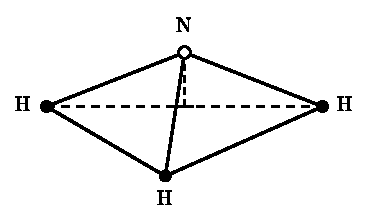
\includegraphics[width=4.5cm]{fig41.pdf}\\[0.3em]{\small 图 41}\end{minipage}\par\nopagebreak

解：这个分子的对称点群为 $\boldsymbol{C}_{3v}$.绕三阶轴旋转只有一个原子（N）不动，对 $\sigma_v$ 反射有两个原子不动（N 和一个 H）.根据(100.4)，(100.6)式求得总表示的特征标为：
\begin{center}
\begin{tabular}{ccc}
  $E$ & $2C_3$ & $3\sigma_v$\\ \hline
  $6$ & $0$ & $2$\\ \hline
\end{tabular}
\end{center}
把这个表示分解为不可约成分，结果发现含有两个 $A_1$ 表示和两个 E 表示.因此有两个无简并的频率对应于两个 $A_1$ 型的振动，保持着该分子的全部对称性（称为完全对称的振动），还有两个双重简并的频率，它们的简正坐标按 E 表示变换.

\noindent{\heiti 习题2}\quad 同题1，但为 $\mathrm{H_2O}$ 分子（图42）.

\par\nopagebreak\noindent\begin{minipage}{\linewidth}\centering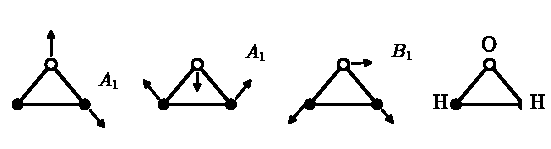
\includegraphics[width=7.5cm]{fig42.pdf}\\[0.3em]{\small 图 42}\end{minipage}\par\nopagebreak

解：对称群为 $\boldsymbol{C}_{2v}$.$C_2$ 变换使 O 原子保持不动，$\sigma_v$ 变换时（对分子平面的反射）三个原子都不动，$\sigma_v'$ 反射时只有 O 原子不动.总振动表示的特征标为：
\begin{center}
\begin{tabular}{cccc}
  $E$ & $C_2$ & $\sigma_v$ & $\sigma_v'$\\ \hline
  $3$ & $1$ & $3$ & $1$\\ \hline
\end{tabular}
\end{center}
这个表示可分解成 $2A_1,1B_1$ 不可约表示，也就是说，存在着两个全对称振动和一个对称性为 $B_1$ 表示的振动，所有的频率都是无简并的.图42中画出了三个相应的简正振动.

\noindent{\heiti 习题3}\quad 同题1，但分子为 $\mathrm{CHCl_3}$（图43a）.

解：分子对称群为 $\boldsymbol{C}_{3v}$.用同一方法我们求得三个 $A_1$ 型的全对称振动和三个 E 型的双重简并振动.

\noindent{\heiti 习题4}\quad 同题1，但分子为 $\mathrm{CH_4}$（C 原子处于四面体的中心，四个 H 原子在顶角，图43b）.

解：分子对称群为 $\boldsymbol{T}_d$，振动为 $1A_1,1E,2F_2$.

\noindent{\heiti 习题5}\quad 同题1，但分子为 $\mathrm{C_6H_6}$（图43c）.

解：分子对称群为 $\boldsymbol{D}_{6h}$.振动为：
\begin{equation*}
\begin{aligned}
  &2A_{1g},\ 1A_{2g},\ 1A_{2u},\ 1B_{1g},\ 1B_{1u},\ 1B_{2g},\ 3B_{2u},\\
  &1E_{1g},\ 3E_{1u},\ 4E_{2g},\ 2E_{2u}.
\end{aligned}
\end{equation*}

\noindent{\heiti 习题6}\quad 同题1，但分子为 $\mathrm{OsF_8}$（Os 原子在立方体的中心，F 原子在顶角上，图43d）.

解：分子对称群为 $\boldsymbol{O}_h$，振动为：
\begin{equation*}
  1A_{1g},\ 1A_{2u},\ 1E_g,\ 1E_u,\ 2F_{1u},\ 2F_{2g},\ 2F_{2u}
\end{equation*}

\noindent{\heiti 习题7}\quad 同题1，但为 $\mathrm{UF_6}$ 分子（U 原子处于八面体中心，F 原子在顶角上，图43e）.

解：分子对称群为 $\boldsymbol{O}_h$，振动为：
\begin{equation*}
  1A_{1g},\ 1E_g,\ 2F_{1u},\ 1F_{2g},\ 1F_{2u}.
\end{equation*}

\par\nopagebreak\noindent\begin{minipage}{\linewidth}\centering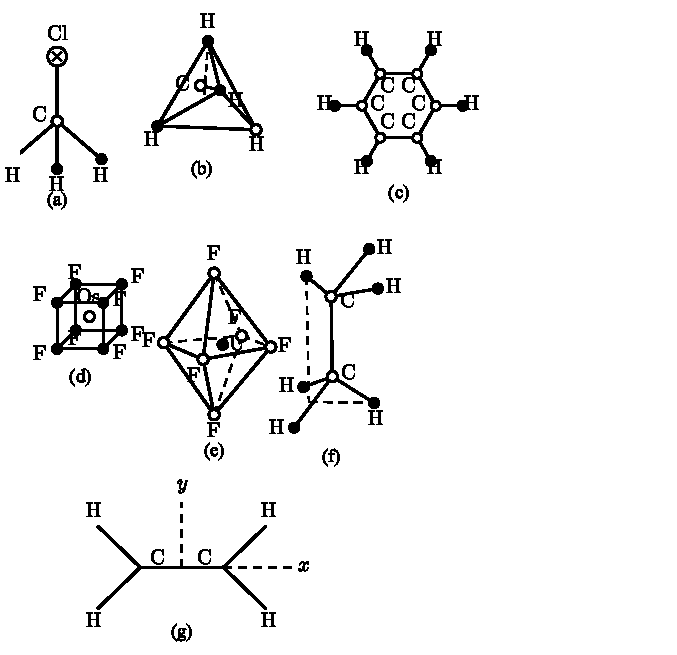
\includegraphics[width=10.5cm]{fig43.pdf}\\[0.3em]{\small 图 43}\end{minipage}\par\nopagebreak

\noindent{\heiti 习题8}\quad 同题1，但分子为 $\mathrm{C_2H_6}$（图43f）.

解：分子对称群为 $\boldsymbol{D}_{3d}$，振动为：
\begin{equation*}
  3A_{1g},\ 1A_{1u},\ 2A_{2u},\ 3E_g,\ 3E_u.
\end{equation*}

\noindent{\heiti 习题9}\quad 同题1，但分子为 $\mathrm{C_2H_4}$（图43g；所有原子在同一平面内）.

解：分子对称群为 $\boldsymbol{D}_{2h}$.振动为：
\begin{equation*}
  3A_{1g},\ 1A_{1u},\ 2B_{1g},\ 1B_{1u},\ 2B_{3u},\ 1B_{2g},\ 2B_{2u}.
\end{equation*}
（所取的坐标轴见该图）.

\noindent{\heiti 习题10}\quad 同题1，但为一线型分子，由 $N$ 个原子所组成并且对称于它的中点.

解：除了本节所讲的线型分子的振动分类外，还需要考虑对中点反演的性质.存在着两种不同的情况，要看 $N$ 是偶数还是奇数.

如果 $N$ 是偶数（$N=2p$），该分子的中点处就不存在原子.给出了该分子半截 $p$ 个原子沿轴线的独立位移后，可令其余的 $p$ 个原子具有与前者相等和相反的位移，结果就有 $p$ 个振动使诸原子保持在轴线上并且对称于它的中点，其余的 $(2p-1)-p=p-1$ 个共线振动对中点则是反对称的.此外，$p$ 个原子不处于同一直线上的运动自由度为 $2p$.我们令对称置放的原子具有相等和相反的位移，就得到 $2p$ 个对称的振动，但在其中必须扣掉相当于分子转动的两个自由度.因此共有 $p-1$ 个双重简并的频率使得原子离轴振动并且对称于它的中点，其余 $(2p-2)-(p-1)=p-1$ 个双重简并频率相当于对中点反对称的振动.应用 $\boldsymbol{D}_{\infty h}$ 群不可约表示的名称（见§98末段），我们可以说，$A_{1g}$ 型的振动有 $p$ 个，$A_{1u}$，$E_{1g},E_{1u}$ 型的振动各有 $p-1$ 个.

如果 $N$ 是奇数（$N=2p+1$），经过类似的分析可以证明，$A_{1g},A_{1u},E_{1u}$ 型的振动各有 $p$ 个而 $E_{1g}$ 型的振动有 $p-1$ 个.

\end{xiti}

\section{振动能级}

从量子力学的观点看来，分子的振动能量由下列哈密顿量的本征值所确定：
\begin{equation}
  \hat{H}^{(v)}=\frac{1}{2}\sum_{\alpha}\sum_{i=1}^{f_\alpha}\hat{P}_{\alpha i}^2
  +\frac{1}{2}\sum_{\alpha}\omega_\alpha^2\sum_{i=1}^{f_\alpha}Q_{\alpha i}^2,
\end{equation}
式中的 $\hat{P}_{\alpha i}=-\mathrm{i}\hbar\dfrac{\partial}{\partial Q_{\alpha i}}$ 是简正坐标 $Q_{\alpha i}$ 所对应的动量算符.由于这个哈密顿量可以分解成独立项 $(\hat{P}_{\alpha i}^2+\omega_\alpha^2Q_{\alpha i}^2)$ 之和，它的能级就可以表成下列求和式：
\begin{equation}
  E^{(v)}=\hbar\sum_{\alpha}\omega_\alpha\sum_i\left(v_{\alpha i}+\frac{1}{2}\right)
  =\sum_{\alpha}\hbar\omega_\alpha\left(v_\alpha+\frac{f_\alpha}{2}\right),
\end{equation}
式中的 $v_\alpha=\sum_i v_{\alpha i}$，$f_\alpha$ 是频率 $\omega_\alpha$ 的多重度.它的波函数等于相应线性谐振子波函数的乘积：
\begin{equation}
  \psi=\prod_{\alpha}\psi_\alpha,
\end{equation}
\begin{equation}
  \psi_\alpha=\text{常数}\times
  \exp\Big(-\frac{1}{2}c_\alpha^2\sum_i Q_{\alpha i}^2\Big)
  \prod_i H_{v_{\alpha i}}(c_\alpha Q_{\alpha i}).
\end{equation}
$H_v$ 代表 $v$ 阶厄米多项式，$c_\alpha=\sqrt{\omega_\alpha/\hbar}$.如果 $\omega_\alpha$ 中存在着多重频率，振动能级一般讲来是简并的.(101.2)式中的能量仅依赖于求和 $v_\alpha=\sum_i v_{\alpha i}$.因此能级简并度等于用 $v_{\alpha i}$ 凑成一组给定 $v_\alpha$ 的拼凑方式数.对于单个 $v_\alpha$ 讲来，拼凑方式数为\footnote{等于 $v_\alpha$ 个球放到 $f_\alpha$ 个匣子中的置放方式数.}
\begin{equation*}
  \frac{(v_\alpha+f_\alpha-1)!}{v_\alpha!\,(f_\alpha-1)!}.
\end{equation*}
因此总简并度为：
\begin{equation}
  \prod_{\alpha}\frac{(v_\alpha+f_\alpha-1)!}{v_\alpha!\,(f_\alpha-1)!}.
\end{equation}
对于双重简并的频率，这个乘积中的因子等于 $v_\alpha+1$，三重简并频率的因子则为 $\dfrac{1}{2}(v_\alpha+1)(v_\alpha+2)$.

必须指出的是，以上的简并度仅仅对纯粹的谐振动才成立.当我们在哈密顿量中考虑了简正坐标的更高次幂（非谐振动）以后，这个简并会被解除，即使不是完全的解除（进一步讨论见§104）.

属于同一简并振动谱项的一组(101.3)式的波函数，给出了分子对称群的某个表示（这个表示一般是可约的）.但是，属于不同频率的函数组是相互独立变换的.因此由(101.3)式的所有波函数给出的一个表示，等于由(101.4)式的函数组所给出的各个表示的直积，所以我们只要研究后一种表示就可以了.

(101.4)式中的指数因子对所有的对称变换保持不变.在厄米多项式中，只有幂次相同的项能够进行相互变换（对称变换显然不会改变每项的幂次）.另一方面，每一厄米多项式完全由它的最高次项所决定，即可写作
\begin{equation*}
  \sum_{i=1}^{f_\alpha}H_{v_{\alpha i}}(c_\alpha Q_{\alpha i})
  =\text{常数}\cdot Q_{\alpha 1}^{v_{\alpha 1}}Q_{\alpha 2}^{v_{\alpha 2}}
  \cdots Q_{\alpha f_\alpha}^{v_{\alpha f_\alpha}}+\text{低次项，}
\end{equation*}
因此我们只要考虑最高次项就可以了.

\emergencystretch=2em%
具有相同 $v_\alpha=\sum_i v_{\alpha i}$ 值的各个函数属于同一谱项.因此把 $v_\alpha$ 个 $Q_{\alpha i}$ 相乘起来，它们的各种乘积可以给出一个表示，这个表示就是以 $Q_{\alpha i}$ 为基的不可约表示的 $v_\alpha$ 次对称乘积（见§94）（L.Tisza,1933）.

\emergencystretch=0pt%


对于一维表示，它的 $v$ 次对称乘积的特征标显然是\footnote{我们采用 $\chi_v(G)$ 记号代替不方便的 $[\chi^v](G)$.}
\begin{equation*}
  \chi_v(G)=[\chi(G)]^v.
\end{equation*}
对二维和三维表示讲来，最好应用以下的数学技巧.\footnote{这个办法是由 А.~С.~Компанейц（1940）采用的.}不可约表示各个基函数的平方和对所有的对称变换保持不变.因此可以把这组基函数形式地看作是一个二维或三维矢量的各个分量，并把对称变换看作是作用在这个矢量上的某种旋转（或反射）.需要强调的是，这样的旋转和反射不能和实际的对称变换混为一谈，它们（对于每一个给定的群元 $G$）还依赖于所考虑的表示.

我们进一步考虑二维表示.设 $\chi(G)$ 为所给二维表示中某一群元的特征标，且有 $\chi(G)\neq0$.一个二维矢量在平面中旋转 $\varphi$ 角后，它的 $x,y$ 分量的变换矩阵的对角元之和等于 $2\cos\varphi$.如令
\begin{equation}
  2\cos\varphi=\chi(G),
\end{equation}
我们就可以求出这个不可约表示中群元 $G$ 形式上所对应的转角 $\varphi$.这个表示自身的 $v$ 次对称乘幂，是由 $v+1$ 个基函数 $x^v,x^{v-1}y,\cdots,y^v$ 给出的.这个 $v$ 次对称乘幂表示的特征标为\footnote{计算 $\chi_v(G)$ 时最好采用下列形式的基函数：
\begin{equation*}
  (x+\mathrm{i}y)^v,\ (x+\mathrm{i}y)^{v-1}(x-\mathrm{i}y),\cdots,(x-\mathrm{i}y)^v,
\end{equation*}
此时的旋转变换矩阵是对角的，对角元之和为：
\begin{equation*}
  \mathrm{e}^{\mathrm{i}v\varphi}+\mathrm{e}^{\mathrm{i}(v-2)\varphi}+\cdots+\mathrm{e}^{-\mathrm{i}v\varphi}.
\end{equation*}}
\begin{equation}
  \chi_v(G)=\frac{\sin(v+1)\varphi}{\sin\varphi}.
\end{equation}
$\chi(G)=0$ 的情形需要特殊的考虑，因为零特征标既可能是旋转 $\pi/2$ 角也可能是反射.如果 $\chi(G^2)=-2$，则为旋转 $\pi/2$ 角，而 $\chi_v(G)$ 为：
\begin{equation}
  \chi_v(G)=(-1)^{v/2}\frac{1+(-1)^v}{2}.
\end{equation}
如果 $\chi(G^2)=2$，则 $\chi(G)$ 必须看作反射（即 $x\longrightarrow x,y\longrightarrow-y$ 的变换）的特征标，此时
\begin{equation}
  \chi_v(G)=\frac{1+(-1)^v}{2},
\end{equation}
同法可得三维表示对称乘幂的特征标公式.所给表示中群元所对应的那种形式上的旋转或反射，很容易利用表7（§95）求出.这种形式上的变换，就是坐标系按所给表示变换的那个同构群中与所给 $\chi(G)$ 值相对应的那个变换.例如对于 $\boldsymbol{O}$ 群和 $\boldsymbol{T}_d$ 群的 $F_1$ 表示，我们应取 $\boldsymbol{O}$ 群的变换；但对于这两个群的 $F_2$ 表示，我们应取 $\boldsymbol{T}_d$ 群的变换.它们的特征标 $\chi_v(G)$ 我们不在这里推导.

\section{分子对称位形的稳定性}

当原子核具有对称位形时，如果对称群具有一个或一个以上的维数大于1的不可约表示，则分子的一个电子谱项有可能是简并的.我们要问，这样的对称位形是不是该分子的一个稳定平衡位形.我们完全不考虑自旋的影响（如果它存在的话），因为这种影响在多原子分子中通常可以略去不计.我们要讲的电子谱项简并性因此和自旋无关，仅仅是轨道简并性.

如果所给位形是稳定的，作为核距函数的分子能量在所给位形下必是一极小值.这就意味着，原子核小位移时，能量的改变式中不能含有这种位移的线性项.

设 $\hat{H}$ 为该分子电子态的哈密顿算符，原子核的间距是它的一些参量.当原子核具有所给的对称位形时，我们把这个哈密顿算符记作 $\hat{H}_0$.可以取简正振动坐标 $Q_{\alpha i}$ 作为确定原子核小位移的各个量.把 $\hat{H}$ 展成 $Q_{\alpha i}$ 的幂级数后可得：
\begin{equation}
  \hat{H}=\hat{H}_0+\sum_{\alpha,i}V_{\alpha i}Q_{\alpha i}
  +\sum_{\alpha,\beta,i,k}W_{\alpha i,\beta k}Q_{\alpha i}Q_{\beta k}+\cdots,
\end{equation}
$V,W,\cdots$ 等展开系数只是电子坐标的函数.在对称变换下，$Q_{\alpha i}$ 诸量变为相互间的组合，此时(102.1)式中的各个和变成同一类型的另一些和.因此我们可以把对称变换形式地看作 $Q_{\alpha i}$ 不变时这些和中的系数的变换.特别是 $V_{\alpha i}$ 系数（给定 $\alpha$ 值的一组系数）将和坐标 $Q_{\alpha i}$ 一样按对称群的同一表示变换.这是因为哈密顿量对所有的对称变换保持不变，它的展式中的每一个齐次项包括线性项在内也将对所有的对称变换保持不变\footnote{严格讲来，$V_{\alpha i}$ 应按 $Q_{\alpha i}$ 的复共轭表示变换.但是正如我们已经指出的，如果这两个复共轭表示并不相同，那么从物理上讲来应该把它们合在一起看成一个维数加倍的表示.所以这个声明并不重要.}.

我们来考虑某个简并的（在对称位形下）电子谱项 $E_0$.原子核的位移破坏了分子的对称性，一般讲来它会引起谱项的分裂.近似到核位移的线性项为止，谱项的分裂值由展开式(102.1)中线性项的矩阵元所组成的一个久期方程所确定，这种矩阵元为
\begin{equation}
  V_{\rho\sigma}=\sum_{\alpha,i}\,Q_{\alpha i}\int\psi_\rho V_{\alpha i}\psi_\sigma\,\mathrm{d}q,
\end{equation}
式中的 $\psi_\rho,\psi_\sigma$ 是属于所考虑简并谱项的电子态的波函数（已选为实函数）.对称位形的稳定性要求与 $Q$ 成正比的分裂值等于零，也就是要求这个久期方程所有 $Q$ 的根全都等于零，这就意味着 $V_{\rho\sigma}$ 矩阵本身必须等于零.当然，我们只应该考虑破坏分子对称性的那些简正振动，也就是说应该把全对称振动（对应于群的单位表示）事先除去.

由于 $Q_{\alpha i}$ 是任意的，所以若(102.2)式的矩阵元等于零则只能是以下的所有积分等于零：
\begin{equation}
  \int\psi_\rho V_{\alpha i}\psi_\sigma\,\mathrm{d}q.
\end{equation}
令 $D^{el}$ 为电子波函数 $\psi_\rho$ 借以变换的不可约表示，$D_\alpha$ 为 $V_{\alpha i}$ 借以变换的不可约表示；我们已经讲过，表示 $D_\alpha$ 就是简正坐标 $Q_{\alpha i}$ 借以变换的那个表示.根据§97中的结论，如果 $[D^{(el)2}]\times D_\alpha$ 中含有单位表示也就是 $[D^{(el)2}]$ 中含有 $D_\alpha$，则(102.3)式的积分不等于零.反之则所有的积分都等于零.

由此可见，如果表示 $[D^{(el)2}]$ 中不含有标志分子振动的任何一个 $D_\alpha$ 不可约表示（单位表示除外），所给的对称位形就是稳定的.对于无简并的电子态讲来，这个条件总能得到满足，因为一维表示自身的对称乘幂是一个单位表示.

举 $\mathrm{CH_4}$ 型的分子为例，其中的一个原子（C）处于中心，另四个原子（H）处于四面体的四个顶角上.这样的位形具有 $\boldsymbol{T}_d$ 对称性.简并电子谱项相当于这个群中的 $E,F_1,F_2$ 表示.该分子具有一个 $A_1$ 型简正振动（全对称振动），一个 E 型双重简并振动和两个 $F_2$ 型三重简并振动（见§100，题4）.$E,F_1,F_2$ 自身的对称乘积为
\begin{equation*}
  [E^2]=A_1+E,\qquad[F_1^2]=[F_2^2]=A_1+E+F_2.
\end{equation*}
我们看到，每个中至少含有一个 E 或 $F_2$ 表示，因此对简并电子态讲来所考虑的四面体位形是不稳定的.

这个结论构成一个普遍规律，称为杨-特勒定理（H.A.Jahn，E.Teller，1937）：当存在简并电子态时，原子核的任何对称位形（共线时除外）都是不稳定的.由于这种不稳定性，原子核以破坏这种对称位形的方式运动，以使谱项的简并性完全解除.我们可以这样说，一个对称（非共线的）分子的电子基项只能是非简并的.\footnote{由于同一对称性导致的简并电子态中的对称性遭受破坏这一物理概念是由朗道（1934）提出的.杨和特勒考虑了分子中所有可能的各种原子核对称位形并用以上方法逐个加以考察后证明了这个定理.}.

刚才讲过线型分子是一个例外.这一点不用群论也易证明.原子核的离轴位移是具有 $\xi$ 和 $\eta$ 分量的一个普通矢量（$\zeta$ 轴沿分子轴）.我们在§87中看到，这种矢量的矩阵元中只有角动量的轴分量 $\Lambda$ 值改变1的那些跃迁矩阵元才不等于零.另一方面，线型分子简并谱项的两个态分别具有角动量轴分量值 $\Lambda$ 和 $-\Lambda$（$\Lambda\geqslant1$）.这两个态间的跃迁至少要使 $\Lambda$ 的改变值等于2，因此矩阵元总是等于零.由此可见，分子中原子核的共线位形有可能是稳定的，即使电子态为简并也是一样.

对定理的一个建设性的普遍证明出于以下的考虑（E.Ruch,1957）.由于原子核的位形对称性而导致的电子态的简并，仅当分子的对称点群中至少出现一个阶数 $n>2$ 的旋转 $(C_n)$ 轴或旋转-反射 $(S_n)$ 轴时才有此可能.此时相互简并态的波函数（即表示 $D^{(el)}$ 的那些基函数）中至少有一个波函数的电子密度 $\rho=|\psi|^2=\psi^2$ 对该轴不是旋转不变的，电子的电场将和电子密度一样对该轴也不对称.在一个（非共线）分子中，存在着一些不在轴上的等价核，在 $C_n$ 或 $S_n$ 旋转下相互易位.因此从电场看来这些等价核所处的位置是不等价的.但是电场内一组带电粒子的各个平衡位置的等价性并不需要电场本身的对称性，这样的事是不可能的，除非是巧合.

\emergencystretch=2em%
对定理的系统证明不过是上述物理情况的一种数学具体化.让我们来指出这个证明的结构（E.Ruch，A.Sch\"onhofer,1965）\footnote{详见 E.~Ruch, A.~Sch\"onhofer, Theoret. chim. acta (Berl.). 1965. Bd.~3. S.~291.}.

\emergencystretch=0pt%


我们来考虑（非线型分子中）某个核 $a$，它不在分子的“中心”上（即不在群中对称变换的固定点上）；也不在对称主轴上，如果有这样的主轴的话\footnote{所谓主轴是指（立方体群和二十面体群以外的对称群中）$n>2$ 的 $C_n$ 或 $S_n$ 轴.}.设 $\boldsymbol{H}$ 为保持核 $a$ 不动的所有分子对称变换的集合，$\boldsymbol{H}$ 是分子总对称群 $\boldsymbol{G}$ 的一个子群，它可能是 $\boldsymbol{C}_1,\boldsymbol{C}_s,\boldsymbol{C}_n,\boldsymbol{C}_{nv}$ 诸点群之一.在 $\boldsymbol{G}$ 中而不在 $\boldsymbol{H}$ 中的那些变换把核 $a$ 变到其它等价核 $a',a'',\cdots$ 的位置上去.设 $s$ 为这组等价核的数目，子群 $\boldsymbol{H}$ 的阶显然等于 $g/s$，$g$ 是整群 $\boldsymbol{G}$ 的阶（即 $s$ 为子群 $\boldsymbol{H}$ 在群 $\boldsymbol{G}$ 中的指数）\footnote{群 $\boldsymbol{G}$ 的所有元可以分成 $S$ 个陪集 $\boldsymbol{H},G'\boldsymbol{H},G''\boldsymbol{H},\cdots$，其中 $G',G'',\cdots$ 是把核 $a$ 变换到 $a',a'',\cdots$ 的元.}.

$s$ 的数目至少是3.因为维数大于1的不可约表示 $D^{(el)}$ 的存在，至少要有一个阶数高于2的对称轴（已经讲过），根据所述条件，核 $a$ 不在这个主轴上.

群 $\boldsymbol{G}$ 的表示 $D^{(el)}$ 对于对称性较低的群 $\boldsymbol{H}$ 而言一般是可约的.我们假定它分解成为 $\boldsymbol{H}$ 的不可约表示时含有一个维数为1的表示 $d^{(el)}$.它是由一个电子波函数 $\psi$ 给出的，$\psi$ 是 $D^{(el)}$ 表示的基函数之一.由于 $d^{(el)}$ 的维数为1，$\rho=\psi^2$ 对 $\boldsymbol{H}$ 中的所有变换保持不变，也就是给出了该群的一个单位不可约表示.

$\boldsymbol{H}$ 的这种单位表示也可以用原子 $a$ 的位移之一 $Q_a$ 为基矢得到，这个位移沿着从分子中心到核 $a$ 的径矢.

对这个位移施行 $\boldsymbol{G}$ 中的所有操作后，得到群 $\boldsymbol{G}$ 的一个 $D_Q$ 表示（一般为可约）的基函数组.由于在 $\boldsymbol{G}$ 中而不在 $\boldsymbol{H}$ 中的每个变换把位移 $Q_a$ 变换到其它 $s-1$ 个等价核 $a',a'',\cdots$ 中的一个位移上，而不同核的位移当然是线性独立的，所以 $D_Q$ 的维数为 $s$.构成 $D_Q$ 基函数组的位移 $Q_a,Q_{a'},\cdots$ 肯定地不能对应于整个分子的移动或转动：如果有三个或更多个等价核的话，它们的径向位移不能组合成为分子的这些位移.

同理，对函数 $\rho=\psi^2$ 施行所有变换后可得群 $\boldsymbol{G}$ 的一个表示 $D_\rho$.$D_\rho$ 的维数可能是 $s$ 也可能小于 $s$，因为我们没有理由假定 $s$ 个函数 $\rho,G'\rho,G''\rho,\cdots$ 都是线性独立的.但是我们可以说，如果表示 $D_\rho$ 不同于 $D_Q$，那么它一定整个地包含在 $D_Q$ 内\footnote{这个论断的含义如下.设子群 $\boldsymbol{H}$ 的一个表示（维数为 $f$）是由几套不同的基函数组给出的，并设对其中的一套施行 $\boldsymbol{G}$ 中的所有变换后给出 $\boldsymbol{G}$ 的一个 $sf$ 维表示，$s$ 是子群 $\boldsymbol{H}$ 在 $\boldsymbol{G}$ 中的指数.那么我们就可以这样说，对任何其它一套基函数组施行同样的变换后所得的一个 $\boldsymbol{G}$ 群表示，或者和前一个表示相同或者完全包含在前一个表示之内，严格证明见371页的脚注②.}.此外，它一定不是单位表示，因为 $\psi^2$ 对整群 $\boldsymbol{G}$ 而言肯定不是不变的；只有维数超过1的不可约表示 $D^{(el)}$ 的基函数的平方和才是不变的.

表示 $D_Q$ 和 $D_\rho$ 的这些性质立刻能给出所需的结论：$D_Q$ 是总振动表示的一部分，$D_\rho$ 是 $[D^{(el)2}]$ 表示的一部分，不含单位表示.$D_Q$ 中包含了 $D_\rho$，这就说明了 $[D^{(el)2}]$ 中至少含有一个非单位振动表示 $D_\alpha$，这正是我们要证明的.

上述论证中，我们假定了 $D^{(el)}$ 分解成为子群 $\boldsymbol{H}$ 的不可约表示时含有一个维数为1的表示.这个假定在绝大多数情况下是正确的.例如，当 $\boldsymbol{H}=\boldsymbol{C}_1,\boldsymbol{C}_s,\boldsymbol{C}_2,\boldsymbol{C}_{2v}$ 时肯定是正确的（因为这些群的所有不可约表示的维数为1）.当 $\boldsymbol{H}=\boldsymbol{C}_n,\boldsymbol{C}_{nv}$ 而 $n>2$ 时也肯定是正确的，只要 $D^{(el)}$ 的维数为奇数（因为 $\boldsymbol{C}_n$ 和 $\boldsymbol{C}_{nv}$ 群只有维数为1或2的不可约表示）.考察点群不可约表示的特征标表以后，可以看到一个例外，这就是立方体群 $\boldsymbol{G}=\boldsymbol{O},\boldsymbol{T}_d,\boldsymbol{O}_h$ 的二维表示相对于子群 $\boldsymbol{H}=\boldsymbol{C}_3,\boldsymbol{C}_{3v}$.

让我们取 $\boldsymbol{G}=\boldsymbol{O}$ 和 $\boldsymbol{H}=\boldsymbol{C}_3$ 这个特例，它只反映表示的名称.两个电子波函数 $\psi_1,\psi_2$ 给出 $\boldsymbol{O}$ 群的 $D^{(el)}=E$ 表示以及子群 $\boldsymbol{C}_3$ 的 $d^{(el)}=E$ 表示，至于 $\boldsymbol{C}_3$，由乘积 $\psi_1^2,\psi_2^2,\psi_1\psi_2$ 给出的表示为 $[E^2]=A+E$.以核 $a$ 的任一位移矢量 $\boldsymbol{Q}_a$ 的三个分量为基，可得同样的 $\boldsymbol{C}_3$ 表示.在这种情形下，$\boldsymbol{O}$ 的 $D_\rho$ 表示为 $[D^{(el)2}]=A_1+E$，不含对应于整个分子移动或转动矢量的 $F_2$ 表示，它同时含有单位表示和一个非单位表示.由于 $D_\rho$ 包含在 $D_Q$（维数为 $3s$）内（理由同前），这就证明了这些情况下分子也是不稳定的\footnote{还有一个例外是二十面体群的4维表示，作类似的处理后得到同样的结论.}.

与本章之初所作的声明相一致，以上的全部讨论中我们把电子态的简并性完全归结为纯轨道的来源.但可指出，即使计及自旋-轨道作用和自旋-自旋作用，杨-特勒定理仍能成立，唯一区别是，在自旋为半整数的（非线型）分子中克拉默斯双重简并不会导致不稳定性，这和§60中证明的普遍定理相一致.后者对应于双点群的二维双值不可约表示.这种情形下之所以没有不稳定性，可以从以下纯形式的论证中看出.在 $D^{(el)}$ 为双值表示的情形下，求(102.3)矩阵元的选择定则时，我们必须考虑反对称乘积 $\{D^{(el)2}\}$ 而不是对称乘积（见§99）.但对维数为2的每个双值不可约表示讲来，反对称乘积均为单位表示，这就是说，这些乘积中肯定不含与分子的任何非全对称振动相对应的那些表示.

\section{陀螺转动的量子化}

在多原子分子转动能级的研究中，往往由于在研究转动时必须同时研究振动而遇到了困难.作为初步例子，让我们把转动的分子看作一个刚体（一个陀螺），亦即具有“刚性联结”的原子.

令 $\xi,\eta,\zeta$ 为一坐标系，它的三个坐标轴沿着陀螺的三个转动惯量主轴并随陀螺一起转动.把经典能量表式中的转动角动量分量 $J_\xi,J_\eta,J_\zeta$，改成相应的算符以后，即得相应的哈密顿量：
\begin{equation}
  \hat{H}=\frac{1}{2}\hbar^2\bigg(\frac{\hat{J}_\xi^2}{I_A}
  +\frac{\hat{J}_\eta^2}{I_B}+\frac{\hat{J}_\zeta^2}{I_C}\bigg),
\end{equation}
式中的 $I_A,I_B,I_C$ 是陀螺的三个主转动惯量.

\emergencystretch=2em%
旋转坐标系中角动量分量算符 $\hat{J}_\xi,\hat{J}_\eta,\hat{J}_\zeta$ 间的对易关系不是那么明显的，因为角动量分量 $\hat{J}_x,\hat{J}_y,\hat{J}_z$ 间的通常对易关系式是在定坐标系中推导出来的.但是，它们很易用以下公式求出

\emergencystretch=0pt%

\begin{equation}
  (\hat{\boldsymbol{J}}\cdot\boldsymbol{a})(\hat{\boldsymbol{J}}\cdot\boldsymbol{b})
  -(\hat{\boldsymbol{J}}\cdot\boldsymbol{b})(\hat{\boldsymbol{J}}\cdot\boldsymbol{a})
  =-\mathrm{i}\hat{\boldsymbol{J}}\cdot(\boldsymbol{a}\times\boldsymbol{b}),
\end{equation}
式中 $\boldsymbol{a},\boldsymbol{b}$ 是标志该刚体的两个任意对易矢量.把上式左边写在 $x,y,z$ 定坐标系中，应用角动量分量间以及它们和任一矢量的分量间的普通对易法则，很易验证以上等式是成立的.

现在设 $\boldsymbol{a}$ 和 $\boldsymbol{b}$ 是沿 $\xi$ 和 $\eta$ 轴的单位矢量.则 $\boldsymbol{a}\times\boldsymbol{b}$ 是沿 $\zeta$ 轴的单位矢量，由(103.2)给出
\begin{equation}
  \hat{J}_\xi\hat{J}_\eta-\hat{J}_\eta\hat{J}_\xi=-\mathrm{i}\hat{J}_\zeta,
\end{equation}
同法可得另外两个对易式.于是旋转坐标系中角动量分量算符的对易式与定坐标系中的区别仅在于式右差了一个符号\footnote{这个事实表明，从所作用的陀螺波函数看来，$x,y,z$ 坐标系的转动等价于 $\xi,\eta,\zeta$ 坐标系的反转动.}.由此可知，根据以前的对易式求得的本征值以及矩阵元等等公式只要一律改成它们的复共轭式，就能对 $J_\xi,J_\eta,J_\zeta$ 适用.特别是 $J_\zeta$ 的本征值（本节中记作 $k$，而 $J_z$ 的本征值记作 $M$）的取值为 $k=-J,\cdots,+J$，$J$ 是一个整数，即陀螺角动量的值.

\subsection*{球型陀螺}

现在来求转动陀螺的能量本征值，最简单的情形是刚体的三个主转动惯量全都相等：$I_A=I_B=I_C=I$.当分子的对称群是一个立方体点群的时候就属于这种情形.(103.1)式的哈密顿量呈下列形式
\begin{equation*}
  \hat{H}=\frac{\hbar^2}{2I}\hat{\boldsymbol{J}}^2,
\end{equation*}
其本征值为
\begin{equation}
  E=\frac{\hbar^2}{2I}J(J+1),
\end{equation}
其中每个能级具有角动量相对于刚体本身的 $2J+1$ 个方向简并性（即 $J_\zeta=k$ 有 $2J+1$ 个值）\footnote{今后我们不再去管角动量沿定坐标轴的 $2J+1$ 重方向简并性，这种简并总是存在的，但在物理上并不重要.如果把这个简并性包括在内，一个球型陀螺的能级总简并度为 $(2J+1)^2$}.

\subsection*{对称陀螺}

当陀螺的主转动惯量只有两个相等时，即 $I_A=I_B\neq I_C$ 时，也不难算出其能级.具有二阶以上对称轴的一个分子就属于这种情形.哈密顿量(103.1)呈下列形式：
\begin{equation}
  \hat{H}=\frac{\hbar^2}{2I_A}\big(\hat{J}_\xi^2+\hat{J}_\eta^2\big)
  +\frac{\hbar^2}{2I_C}\hat{J}_\zeta^2
  =\frac{\hbar^2}{2I_A}\hat{\boldsymbol{J}}^2
  +\frac{1}{2}\hbar^2\left(\frac{1}{I_C}-\frac{1}{I_A}\right)\hat{J}_\zeta^2,
\end{equation}
由此可见，具有确定的 $J$，$k$ 值的态所具有的能量为
\begin{equation}
  E=\frac{\hbar^2}{2I_A}J(J+1)
  +\frac{1}{2}\hbar^2\left(\frac{1}{I_C}-\frac{1}{I_A}\right)k^2,
\end{equation}
此式给出了对称陀螺的能级.

球型陀螺中出现的对 $k$ 值的简并在这里得到了部分的解除.只有符号相反的两个 $k$ 值具有相同的能量，这与角动量沿陀螺轴的两个相反方向相对应.因此对称陀螺的能级（$k\neq0$）都是双重简并的.

因此对称陀螺的定态要用三个量子数来描述：角动量 $J$ 及其沿陀螺轴的分量（$J_\zeta=k$）以及沿空间固定的 $z$ 轴的分量（$J_z=M$）；陀螺的能量与最后一个量子数无关.角动量及其沿空间固定轴的分量，以及沿刚性联结于一个物理系统上的轴分量\footnote{不要和沿两个空间固定轴的分量混淆起来（这两个分量不能同时测量）.}，三者之间所以能同时测量是由于算符 $\hat{\boldsymbol{J}}^2$ 和 $J_z$ 不但能相互对易而且还和算符 $\hat{J}_\zeta=\hat{\boldsymbol{J}}\cdot\boldsymbol{n}$ 对易，$\boldsymbol{n}$ 是沿 $\zeta$ 轴的单位矢量.这一点可通过直接计算加以证明，但也能事先知道：角动量算符是一个无限小转动算符，而固定于陀螺上的两个矢量的标积 $\boldsymbol{J}\cdot\boldsymbol{n}$ 对坐标轴的任意转动是不变的.

求对称陀螺的定态波函数于是就变成了求 $\hat{\boldsymbol{J}}^2,J_z$ 和 $\hat{J}_\zeta$ 算符的共同本征函数.这在数学上又和角动量本征函数在有限转动下的变换规律有关.改变量子数的记号以后，(58.7)式的规律可写成
\begin{equation}
  \psi_{JM}=\sum_k D^{(J)}_{kM}(\alpha,\beta,\gamma)\psi_{Jk}.
\end{equation}
我们取 $\psi_{JM}$ 为用定坐标 $x,y,z$ 描述的陀螺状态波函数，$\psi_{Jk}$ 为用附着在陀螺上的坐标轴 $\xi,\eta,\zeta$ 描述的状态波函数.在和物理系统（例如陀螺）刚性连结的坐标系中，$\psi_{Jk}$ 具有与系统的空间方向无关的定值 $\psi_{Jk}^{(0)}$.(103.7)式给出了 $\psi_{JM}$ 对角度的依赖关系.设 $|JM\rangle$ 态还具有确定的沿 $\zeta$ 轴的角动量分量值 $k$.这意味着只有具有这个 $k$ 值的 $\psi_{Jk}^{(0)}$ 才不等于零，于是(103.7)的求和式中只剩下一项
\begin{equation*}
  \psi_{JMk}=\psi_{Jk}^{(0)}D^{(J)}_{kM}(\alpha,\beta,\gamma).
\end{equation*}
上式给出了状态波函数 $|JMk\rangle$ 和欧拉角的关系，这些欧拉角定义了陀螺转轴和固定轴的关系.采用下列波函数归一化条件：
\begin{equation*}
  \int|\psi_{JMk}|^2\sin\beta\,\mathrm{d}\alpha\,\mathrm{d}\beta\,\mathrm{d}\gamma=1,
\end{equation*}
我们有
\begin{equation}
  \psi_{JMk}=\mathrm{i}^J\sqrt{\frac{2J+1}{8\pi^2}}\,
  D^{(J)}_{kM}(\alpha,\beta,\gamma),
\end{equation}
式中的相因子是这样选定的，使得 $k=0$ 时(103.8)式的函数变成总角动量为 $J$，分量为 $M$ 的自由（不附着于 $\zeta$ 轴）角动量本征函数，亦即通常的（球谐）函数；参考(58.25)式\footnote{不用有限转动理论直接推导(103.8)式见题1，用(103.8)式的波函数计算各种量的矩阵元见§110 和§87；与双原子分子（无自旋）相应公式的差别仅在于量子数的名称（见§82 第二个附注）.}.

\subsection*{非对称陀螺}

$I_A\neq I_B\neq I_C$ 时，能级的一般表式无法算出.角动量相对于陀螺方向的简并现在完全被解除，对每个给定的 $J$ 值有 $2J+1$ 个无简并的能级.计算这些能级时，我们要从矩阵形式的薛定谔方程出发（O.Klein,1929），做法如下.

$J$ 以及角动量 $\zeta$ 分量具有定值的陀螺状态波函数 $\psi_{Jk}$ 就是上面导出的(103.8)式的函数（为方便计我们略去下标 $M$，因为能量和 $M$ 无关）.在这些状态中，非对称陀螺的能量并不具有定值.另一方面，在定态中 $J_\zeta$ 分量并不具有定值，亦即能级没有确定的 $k$ 值，定态波函数呈下列线性组合形式：
\begin{equation}
  \psi_J=\sum_k c_k\psi_{Jk},
\end{equation}
式中已假定所有的函数具有公共的 $M$ 值，代入薛定谔方程 $\hat{H}\psi_J=E_J\psi_J$ 中，得方程组
\begin{equation}
  \sum_{k'}\big(\langle Jk|H|Jk'\rangle-E\delta_{kk'}\big)c_{k'}=0
\end{equation}
上式有解的条件为以下久期方程：
\begin{equation}
  \bigl|\langle Jk|H|Jk'\rangle-E\delta_{kk'}\bigr|=0,
\end{equation}
此式的根给出陀螺的能级，然后用(103.10)给出使哈密顿量对角化的(103.9)式中的线性组合系数，亦即给出具有给定 $J$ 值（及 $M$ 值）的陀螺定态波函数.计算对这些波函数而言的任何物理量矩阵元，就化成对对称陀螺波函数而言的矩阵元.

算符 $\hat{J}_\xi,\hat{J}_\eta$ 只有 $k$ 值改变1的跃迁矩阵元，而 $\hat{J}_\zeta$ 只有对角元（见(27.13)式，把式中的 $L,M$ 改成 $J,k$）.因此算符 $\hat{J}_\xi^2,\hat{J}_\eta^2,\hat{J}_\zeta^2$ 从而 $\hat{H}$ 只有 $k\rightarrow k$ 或 $k\pm2$ 的跃迁矩阵元.$k$ 的奇态和偶态间没有跃迁矩阵元，这使得 $2J+1$ 次的久期方程立刻分解成 $J$ 次和 $J+1$ 次的两个独立方程.其中一个只含 $k$ 为偶数的跃迁矩阵元，另一方程只含 $k$ 为奇数的跃迁矩阵元.这两个方程都能进一步化成两个次数较低的方程.为此，我们不能用函数组 $\psi_{Jk}$ 定义的矩阵元，而必须用下列函数组定义的矩阵元：
\begin{equation}
\left.\begin{aligned}
  \psi^+_{Jk}&=\frac{1}{\sqrt{2}}\left(\psi_{Jk}+\psi_{J,-k}\right),
  \qquad\psi^+_{J0}=\psi_{J0},\\
  \psi^-_{Jk}&=\frac{1}{\sqrt{2}}\left(\psi_{Jk}-\psi_{J,-k}\right)\ (k\neq0).
\end{aligned}\right\}
\end{equation}
指标 $+$ 和 $-$ 不一样的函数具有不同的对称性（对通过 $\zeta$ 轴的平面所作的反射，会改变 $k$ 的符号），它们之间的跃迁矩阵元因而等于零.因此我们可把久期方程分解成一个对 $(+)$ 态的和一个对 $(-)$ 态的.

具有对易关系(103.3)的哈密顿量(103.1)具有特殊的对称性：它对 $\hat{J}_\xi,\hat{J}_\eta,\hat{J}_\zeta$ 算符中任意两个算符的同时反号保持不变.这种对称性形式地对应于 $\boldsymbol{D}_2$ 群.因此非对称陀螺的能级可按此群的不可约表示分类.从而有四类无简并能级，分别对应于 $A,B_1,B_2,B_3$ 表示（见§95，表7）.

很易确定非对称陀螺的哪些态属于哪个类型.为此，我们必须找出 $\psi_{Jk}$ 和(103.12)式函数的对称性质.这可从(103.8)式直接做起，但从通常的球谐函数做起更为简单，我们注意到，就其对称性质而言，角动量 $\zeta$ 分量具有定值的状态波函数是和下列角动量本征函数一样的：
\begin{equation}
  \psi_{Jk}\sim Y^*_{Jk}(\theta,\varphi)\sim\mathrm{e}^{-\mathrm{i}k\varphi}\Theta_{Jk}(\theta)
\end{equation}
其中 $\theta$，$\varphi$ 是 $\xi,\eta,\zeta$ 坐标轴中的球面角，记号 $\sim$ 代表“变换相同”；(103.13)中取复共轭是由于对易式(103.3)的右边反号.

绕 $\zeta$ 轴转过 $\pi$ 角后（即对称操作 $C_2^{(\zeta)}$），(103.13)式的函数被乘以 $(-1)^k$：
\begin{equation*}
  C_2^{(\zeta)}\colon\psi_{Jk}\longrightarrow(-1)^k\psi_{Jk}
\end{equation*}
操作 $C_2^{(\eta)}$ 可看作反演再加上对 $\xi\zeta$ 平面的一次反射；第一个操作使 $\psi_{Jk}$ 乘以 $(-1)^J$，第二个操作（$\varphi$ 变号）相当于改变 $k$ 的符号.根据函数 $\Theta_{J,-k}$ 的定义(28.6)，我们有
\begin{equation*}
  C_2^{(\eta)}\colon\psi_{Jk}\longrightarrow(-1)^{J+k}\psi_{J,-k}.
\end{equation*}
最后，对操作 $C_2^{(\xi)}=C_2^{(\eta)}C_2^{(\zeta)}$ 得
\begin{equation*}
  C_2^{(\xi)}\colon\psi_{Jk}\longrightarrow(-1)^J\psi_{J,-k}.
\end{equation*}
应用这些变换规则，我们发现函数组(103.12)的态分属于下列各种对称类型：
\begin{equation*}
  \psi^+_{Jk}\left\{\begin{array}{lll}
    J\text{ 偶}, & k\text{ 偶} & A\\
    J\text{ 偶}, & k\text{ 奇} & B_3\\
    J\text{ 奇}, & k\text{ 偶} & B_1\\
    J\text{ 奇}, & k\text{ 奇} & B_2
  \end{array}\right.
\end{equation*}
\begin{equation}
  \psi^-_{Jk}\left\{\begin{array}{lll}
    J\text{ 偶}, & k\text{ 偶} & B_1\\
    J\text{ 偶}, & k\text{ 奇} & B_2\\
    J\text{ 奇}, & k\text{ 偶} & A\\
    J\text{ 奇}, & k\text{ 奇} & B_3
  \end{array}\right.
\end{equation}
对于一个给定的 $J$ 值，很易算出每一类型中的态数.$A$ 型及每个 $B_1,B_2,B_3$ 型中的态数如下：
\begin{equation}
\begin{array}{|c|c|c|}
\hline
  & A & B_1,\ B_2,\ B_3\\ \hline
  J\text{ 偶} & \frac{1}{2}J+1 & \frac{1}{2}J\\ \hline
  J\text{ 奇} & \frac{1}{2}J-\frac{1}{2} & \frac{1}{2}J+\frac{1}{2}\\ \hline
\end{array}
\end{equation}
对于非对称陀螺，存在着 $A,B_1,B_2,B_3$ 型各态间跃迁矩阵元的选择定则：这些规则很易用通常的对称性考虑得到.对于物理矢量 $\boldsymbol{A}$ 的分量讲来，我们有下列选择定则：
\begin{equation}
\begin{array}{ll}
  A_\xi\colon & A\leftrightarrow B_3^{(\xi)},\ B_1^{(\zeta)}\leftrightarrow B_2^{(\eta)},\\
  A_\eta\colon & A\leftrightarrow B_2^{(\eta)},\ B_1^{(\zeta)}\leftrightarrow B_3^{(\xi)},\\
  A_\zeta\colon & A\leftrightarrow B_1^{(\zeta)},\ B_2^{(\eta)}\leftrightarrow B_3^{(\xi)}
\end{array}
\end{equation}
为清楚起见，群表示的符号上标注了一个坐标轴，绕该轴旋转时所注表示的特征标为 $+1$.

\begin{xiti}
\setcounter{equation}{0}\renewcommand{\theequation}{\arabic{equation}}%

\noindent{\heiti 习题1}\quad 通过直接计算算符 $\hat{\boldsymbol{J}}^2,\hat{J}_z,\hat{J}_\zeta$ 的共同本征函数，求出对称陀螺的 $|JMk\rangle$ 态波函数（F.~Reich\'e,~H.~Rademacher,~1926）.

解：为了求出作为欧拉角 $\alpha,\beta,\gamma$ 的函数的 $\psi_{JMk}$，我们必须用欧拉角表出沿定轴 $x,y,z$ 的角动量分量算符.由于沿任一轴的角动量分量算符为 $-\mathrm{i}\partial/\partial\varphi$，$\varphi$ 是绕该轴的转角，我们有
\begin{equation*}
  \hat{J}_x=-\mathrm{i}\frac{\partial}{\partial\varphi_x},\qquad
  \hat{J}_y=-\mathrm{i}\frac{\partial}{\partial\varphi_y},\qquad
  \hat{J}_z=-\mathrm{i}\frac{\partial}{\partial\varphi_z},
\end{equation*}
其中 $\varphi_x,\varphi_y,\varphi_z$ 为绕相应轴的转角.对这些角的微商可化成对 $\alpha,\beta,\gamma$ 角的微商，因为无限小转动沿转轴可作矢量相加.图20（§58）用欧拉角表出了无限小转动 $\delta\alpha,\delta\beta,\delta\gamma$ 的矢量方向.取它们沿定轴 $x,y,z$ 的分量，即得绕定轴的转角
\begin{equation*}
\begin{aligned}
  \delta\varphi_x&=-\sin\alpha\,\delta\beta+\cos\alpha\sin\beta\,\delta\gamma,\\
  \delta\varphi_y&=\cos\alpha\,\delta\beta+\sin\alpha\sin\beta\,\delta\gamma,
\end{aligned}
\end{equation*}
\begin{equation*}
  \delta\varphi_z=\delta\alpha+\cos\beta\,\delta\gamma.
\end{equation*}
反过来有
\begin{equation*}
\begin{aligned}
  \delta\alpha&=-\cot\beta\cos\alpha\,\delta\varphi_x
  -\cot\beta\sin\alpha\,\delta\varphi_y+\delta\varphi_z,\\
  \delta\beta&=-\sin\alpha\,\delta\varphi_x+\cos\alpha\,\delta\varphi_y,\\
  \delta\gamma&=\frac{\cos\alpha}{\sin\beta}\,\delta\varphi_x
  +\frac{\sin\alpha}{\sin\beta}\,\delta\varphi_y.
\end{aligned}
\end{equation*}
从这些表式得
\begin{equation*}
\begin{aligned}
  \hat{J}_x&=-\mathrm{i}\left(-\cos\alpha\cot\beta\frac{\partial}{\partial\alpha}
  -\sin\alpha\frac{\partial}{\partial\beta}
  +\frac{\cos\alpha}{\sin\beta}\frac{\partial}{\partial\gamma}\right),\\
  \hat{J}_y&=-\mathrm{i}\left(-\sin\alpha\cot\beta\frac{\partial}{\partial\alpha}
  +\cos\alpha\frac{\partial}{\partial\beta}
  +\frac{\sin\alpha}{\sin\beta}\frac{\partial}{\partial\gamma}\right),\\
  \hat{J}_z&=-\mathrm{i}\frac{\partial}{\partial\alpha}.
\end{aligned}
\end{equation*}
当把算符 $\hat{J}_z=-\mathrm{i}\partial/\partial\alpha$ 和 $\hat{J}_\zeta=-\mathrm{i}\partial/\partial\gamma$（$\gamma$ 为绕 $\zeta$ 轴的转角）作用在 $\psi_{JMk}$ 上后，这些算符分别被 $M$ 和 $k$ 所代替（波函数与 $\alpha$ 和 $\gamma$ 角的关系是由因子 $\exp(\mathrm{i}\alpha M+\mathrm{i}\gamma k)$ 给出的）.从而有
\begin{equation*}
\begin{aligned}
  \hat{J}_+&=\hat{J}_x+\mathrm{i}\hat{J}_y
  =\mathrm{e}^{\mathrm{i}\alpha}\left(\frac{\partial}{\partial\beta}
  -M\cot\beta+\frac{k}{\sin\beta}\right),\\
  \hat{J}_-&=\hat{J}_x-\mathrm{i}\hat{J}_y
  =\mathrm{e}^{-\mathrm{i}\alpha}\left(-\frac{\partial}{\partial\beta}
  -M\cot\beta+\frac{k}{\sin\beta}\right).
\end{aligned}
\end{equation*}
剩下的推导和§28末完全一样.我们从方程 $\hat{J}_+\psi_{JJk}=0$ 出发，此式对 $M=J$ 的波函数成立，从而有
\begin{equation*}
  \left(\frac{\partial}{\partial\beta}-J\cot\beta+\frac{k}{\sin\beta}\right)\psi_{JJk}=0,
\end{equation*}
上式的归一化解为
\begin{equation*}
  \psi_{JJk}=\mathrm{i}^J(-1)^{J-k}
  \sqrt{\frac{(2J+1)!}{2(J+k)!(J-k)!}}
  \left(\cos\frac{1}{2}\beta\right)^{J+k}
  \left(\sin\frac{1}{2}\beta\right)^{J-k}
  \frac{1}{2\pi}\mathrm{e}^{\mathrm{i}(J\alpha+k\gamma)}.
\end{equation*}
归一化积分是一个欧拉 $\beta$ 函数.上式除了一个相因子外，实际上与下式相同（参考(58.26)）：
\begin{equation*}
  \sqrt{\frac{2J+1}{8\pi^2}}\,D^{(J)}_{kJ}(\alpha,\beta,\gamma).
\end{equation*}
所选的相因子与(103.7)中的定义一致.

对 $\psi_{JJk}$ 反复应用下式就可算出 $M<J$ 的各个波函数
\begin{equation*}
  \hat{J}_-\psi_{J,M+1,k}
  =\sqrt{(J-M)(J+M+1)}\,\psi_{JMk}.
\end{equation*}
最后结果与(103.8)相同，该处的函数 $D^{(J)}_{kM}$ 为(58.10)和(58.11)式，并计及了这些函数的对称性质(58.18).

\noindent{\heiti 习题2}\quad 计算非对称陀螺的 $\langle Jk'|H|Jk\rangle$ 矩阵元.

解：根据(27.13)式得
\begin{equation*}
\begin{aligned}
  &\langle k|J_\xi^2|k\rangle=\langle k|J_\eta^2|k\rangle
  =\frac{1}{2}\left[J(J+1)-k^2\right],\\
  &\langle k|J_\xi^2|k+2\rangle=\langle k+2|J_\xi^2|k\rangle
  =-\langle k|J_\eta^2|k+2\rangle=-\langle k+2|J_\eta^2|k\rangle\\
  &\qquad\qquad=\frac{1}{4}\left[(J-k)(J-k-1)(J+k+1)(J+k+2)\right]^{\frac{1}{2}},
\end{aligned}
\end{equation*}
为简洁计，矩阵元中一律省略了对角指标 $J$，所求的哈密顿量矩阵元因此为\footnote{题2至题5中，采用下列记号使公式简化：
\begin{equation*}
  a=1/I_A,\qquad b=1/I_B,\qquad c=1/I_C.
\end{equation*}}
\begin{equation}
\left.\begin{aligned}
  \langle k|H|k\rangle&=\frac{1}{4}\hbar^2(a+b)\left[J(J+1)-k^2\right]
  +\frac{1}{2}\hbar^2ck^2,\\
  \langle k|H|k+2\rangle&=\langle k+2|H|k\rangle=\\
  &=\frac{1}{8}\hbar^2(a-b)
  \left[(J-k)(J-k-1)(J+k+1)(J+k+2)\right]^{\frac{1}{2}}.
\end{aligned}\right\}
\end{equation}
相对于函数组(103.12)而言的矩阵元，可通过(1)式的矩阵元表出：
\begin{equation}
\left.\begin{aligned}
  \langle k\pm|H|k\pm\rangle&=\langle k|H|k\rangle\ (k\neq1),\\
  \langle 1\pm|H|1\pm\rangle&=\langle 1|H|1\rangle\pm\langle 1|H|-1\rangle,\\
  \langle k\pm|H|k+2,\pm\rangle&=\langle k|H|k+2\rangle\ (k\neq0),\\
  \langle 0+|H|2+\rangle&=\sqrt{2}\,\langle 0|H|2\rangle.
\end{aligned}\right\}
\end{equation}

\noindent{\heiti 习题3}\quad 试求 $J=1$ 的非对称陀螺的能级.

解：三次的久期方程分解成三个线性方程.其中一个给出
\begin{equation}
  E_1=\langle 0+|H|0+\rangle=\frac{1}{2}\hbar^2(a+b),
\end{equation}
根据上式可以立刻写出其它两个能级，因为 $a,b,c$ 三个参量是以对称的方式出现在这个问题中，从而有
\begin{equation}
  E_2=\frac{1}{2}\hbar^2(a+c),\qquad
  E_3=\frac{1}{2}\hbar^2(b+c).
\end{equation}
$E_1,E_2,E_3$ 能级分别属于\footnote{这是根据对称性的考虑.例如能量 $E_1$ 对于参量 $a$ 和 $b$ 是对称的，因此它的态对 $\xi$ 轴和 $\eta$ 轴具有同样的对称性，亦即属于 $B_1$ 型的态.}对称类型 $B_1,B_2,B_3$.这些态的波函数为
$\psi_1=\psi^+_{10},\psi_2=\psi^+_{11},\psi_3=\psi^-_{11}$.

\noindent{\heiti 习题4}\quad 同题2，但 $J=2$.

解：久期方程为5次，分解成为三个线性方程和一个二次方程.从一个线性方程得
\begin{equation}
  E_1=\langle 2-|H|2-\rangle=2\hbar^2c+\frac{1}{2}\hbar^2(a+b),
\end{equation}
这是属于 $B_1$ 型的一个能级.由此立刻可知，一定有 $B_2$ 和 $B_3$ 型的其它两个能级：
\begin{equation*}
  E_2=2\hbar^2b+\frac{1}{2}\hbar^2(a+c),\qquad
  E_3=2\hbar^2a+\frac{1}{2}\hbar^2(b+c)
\end{equation*}
这三个能级具有波函数 $\psi_1=\psi^-_{22},\psi_2=\psi^-_{21},\psi_3=\psi^+_{21}$.

二次方程为
\begin{equation}
  \left|\begin{array}{cc}
    \langle 0+|H|0+\rangle-E & \langle 2+|H|0+\rangle\\
    \langle 2+|H|0+\rangle & \langle 2+|H|2+\rangle-E
  \end{array}\right|=0,
\end{equation}
解出得
\begin{equation}
  E_{4,5}=\hbar^2(a+b+c)\pm\hbar^2
  \sqrt{(a+b+c)^2-3(ab+bc+ca)}
\end{equation}
这两个能级属于 A 型，相应波函数为 $\psi^+_{20}$ 和 $\psi^+_{22}$ 的线性组合.

\noindent{\heiti 习题5}\quad 同题2，但 $J=3$.

解：久期方程为7次，分解成为一个线性方程和三个二次方程.线性方程给出
\begin{equation}
  E_1=\langle 2-|H|2-\rangle=2\hbar^2(a+b+c),
\end{equation}
这是一个属于 A 型的能级.一个二次方程为题4的(6)式，但 $J$ 值不一样.它的根为
\begin{equation}
  E_{2,3}=\frac{5}{2}\hbar^2(a+b)+\hbar^2c
  \pm\hbar^2\sqrt{4(a-b)^2+c^2+ab-ac-bc},
\end{equation}
这是 $B_1$ 型能级.其余能级可从上式置换 $a,b,c$ 后得到.

\noindent{\heiti 习题6}\quad 具有四极矩的一个系统，处于任意的外电场中，求其能级分裂.

解：取张量 $\partial^2\varphi/\partial x_i\partial x_k$ 的三个主轴为坐标系（见§76题3），哈密顿量的四极矩部分可化成
\begin{equation*}
  \hat{H}=A\hat{J}_x^2+B\hat{J}_y^2+C\hat{J}_z^2,\qquad A+B+C=0.
\end{equation*}
由于上式和(103.1)式的哈密顿量在形式上完全类似，本题等价于寻求非对称陀螺的能级，唯一区别是现在系数之和 $A+B+C=0$，并且角动量还可具有半整数值.这些可用同样的方法从头算起，但对整数 $J$ 值可用题3和题5的结果，对前几个 $J$ 值，所得的能级移动值 $\Delta E$ 如下：
\begin{equation*}
  J=1:\qquad\Delta E=-A,\ -B,\ -C;
\end{equation*}
\begin{equation*}
  J=3/2:\qquad\Delta E=\pm\sqrt{\frac{3}{2}(A^2+B^2+C^2)}\ ;
\end{equation*}
\begin{equation*}
  J=2:\qquad\Delta E=3A,\,3B,\,3C,\ \pm\sqrt{6(A^2+B^2+C^2)}.
\end{equation*}
$J=3/2$ 时分裂能级保持双重简并，与克拉默斯定理（§60）一致.

\end{xiti}
\renewcommand{\theequation}{\arabic{section}.\arabic{equation}}%

\section{分子的振动转动相互作用}

迄今为止我们把转动和振动看作分子的两种独立运动.但在实际上，这两种运动的同时存在产生了它们之间的特殊相互作用（E.Teller，L.Tisza，G.Placzek，1932—1933）.

让我们先从线型多原子分子考虑起.一个线型分子可以作两类振动（见§100末段）：频率为无简并的纵振动和频率为双重简并的横振动.现在我们对后一类振动感兴趣.一般来讲，作横振动的分子具有某种角动量.这一点从简单的力学考虑看来是很明显的\footnote{例如，周相差为 $\frac{1}{2}\pi$ 的两个正交横振动，可以看作一个弯折分子绕一纵轴的纯转动.}，但它也能从量子力学的考虑证实.后一种考虑还能使我们求出该角动量在所给振动态中的各种可能值.

我们假定分子中某一双重频率 $\omega_\alpha$ 受到了激发.振动量子数为 $v_\alpha$ 的能级是 $v_\alpha+1$ 重简并的.与该能级对应的是以下 $v_\alpha+1$ 个波函数：
\begin{equation*}
  \psi_{v_{\alpha_1}v_{\alpha_2}}=\text{常数}\times
  \exp\Big[-\frac{1}{2}c_\alpha^2\big(Q_{\alpha_1}^2+Q_{\alpha_2}^2\big)\Big]
  H_{v_{\alpha_1}}(c_\alpha Q_{\alpha_1})
  H_{v_{\alpha_2}}(c_\alpha Q_{\alpha_2})
\end{equation*}
其中 $v_{\alpha_1}+v_{\alpha_2}=v_\alpha$，或者是这些波函数的任意的独立线性组合.与指数因子相乘的那个多项式的总幂次（$Q_{\alpha_1}$ 的幂加上 $Q_{\alpha_2}$ 的幂），对这些函数讲来都是相等的并等于 $v_\alpha$.显然，我们总能选取 $\psi_{v_{\alpha_1}v_{\alpha_2}}$ 的下列线性组合作为基本函数组：
\begin{equation}
\begin{aligned}
  \psi_{v_\alpha l_\alpha}={}&\text{常数}\times
  \exp\Big[-\frac{1}{2}c_\alpha^2\big(Q_{\alpha_1}^2+Q_{\alpha_2}^2\big)\Big]\times\\
  &\times\Big[\big(Q_{\alpha_1}+\mathrm{i}Q_{\alpha_2}\big)^{(v_\alpha+l_\alpha)/2}
  \big(Q_{\alpha_1}-\mathrm{i}Q_{\alpha_2}\big)^{(v_\alpha-l_\alpha)/2}+\cdots\Big].
\end{aligned}
\end{equation}
方括号内是一个确定的多项式，我们只写出了它的最高次项.$l_\alpha$ 是一个整数，可以取 $v_\alpha+1$ 个不同的值 $v_\alpha,v_\alpha-2,v_\alpha-4,\cdots,-v_\alpha$.

横振动的简正坐标 $Q_{\alpha_1},Q_{\alpha_2}$ 是两个离开分子轴的正交位移.绕轴旋转 $\varphi$ 角后，多项式的最高次项（因而整个函数 $\psi_{v_\alpha l_\alpha}$）被乘以
\begin{equation*}
  \exp\Big\{\mathrm{i}\varphi\Big(\frac{v_\alpha+l_\alpha}{2}\Big)
  -\mathrm{i}\varphi\Big(\frac{v_\alpha-l_\alpha}{2}\Big)\Big\}
  =\exp(\mathrm{i}l_\alpha\varphi).
\end{equation*}
由此可见，(104.1)式的函数对应于角动量的轴分量为 $l_\alpha$ 的一个态.

我们得到的结论是，双重频率 $\omega_\alpha$ 被激发的态（具有量子数 $v_\alpha$）中，该分子具有一个能取下列诸值（相对于分子轴）的角动量
\begin{equation}
  l_\alpha=v_\alpha,v_\alpha-2,v_\alpha-4,\cdots,-v_\alpha
\end{equation}
它称为分子的振动角动量.如果有若干个横振动同时被激发，总的振动角动量就等于 $\sum\limits_\alpha l_\alpha$，加上电子轨道角动量以后，给出该分子沿轴的总角动量 $l$.

分子的总角动量 $\boldsymbol{J}$ 不能小于沿轴的角动量（与双原子分子的情形类似），即 $J$ 的取值为
\begin{equation*}
  J=|l|,\ |l|+1,\ \cdots,
\end{equation*}
换句话说，不存在 $J=0,1,\cdots,|l|-1$ 的态.

简谐振动的情形下，能量只和量子数 $v_\alpha$ 有关而与 $l_\alpha$ 无关.考虑非简谐振动以后，振动能级的简并度（对 $l_\alpha$ 值而言的简并度）有所解除.但是，这种解除是不完全的：分裂能级保持着双重简并，$l$ 和所有 $l_\alpha$ 同时改变符号的两个态具有相同的能量.这是因为在能量的下一级近似（简谐振动后的下一级近似）中，出现 $l_\alpha$ 的二次型 $\sum\limits_{\alpha,\beta}g_{\alpha\beta}l_\alpha l_\beta$（$g_{\alpha\beta}$ 是常数）.通过类似于双原子分子中的 $\Lambda$ 双线效应，这种余留的双重简并即可得到解除.

回到非线型分子时，首先要作下列力学性质的说明.对于任意一个多粒子（非线型）系统讲来，就有一个怎样把振动和转动完全区分开来的问题；换句话说，我们怎样去理解一个“非转动的系统”.乍看起来，不存在转动的判据似乎是角动量等于零：
\begin{equation}
  \sum m\boldsymbol{r}\times\boldsymbol{v}=0
\end{equation}
（$\Sigma$ 是对该系统的粒子求和）.但是这个式子的左边并不等于某一坐标函数对时间的全微商.因此这个等式不能通过对时间的积分而表成某一坐标函数等于零的形式.但这正好是合理地定义“纯振动”和“纯转动”这两个概念所需要的.

因此作为无转动的定义，我们必须采用下列条件：
\begin{equation}
  \sum m\boldsymbol{r}_0\times\boldsymbol{v}=0,
\end{equation}
式中 $\boldsymbol{r}_0$ 是粒子平衡位置的径矢.令 $\boldsymbol{r}=\boldsymbol{r}_0+\boldsymbol{u}$，$\boldsymbol{u}$ 是小振动中的位移，我们有 $\boldsymbol{v}=\dot{\boldsymbol{r}}=\dot{\boldsymbol{u}}$.(104.4)式对时间积分后得
\begin{equation}
  \sum m\boldsymbol{r}_0\times\boldsymbol{u}=0.
\end{equation}
该分子的运动可以看作是满足条件(104.5)的纯振动与整个分子转动的组合\footnote{分子的平动一开始就可除去；只要所选的坐标系相对于分子的质心保持不动.}.

把角动量写成以下形式：
\begin{equation*}
  \sum m\boldsymbol{r}\times\boldsymbol{v}
  =\sum m\boldsymbol{r}_0\times\boldsymbol{v}
  +\sum m\boldsymbol{u}\times\boldsymbol{v},
\end{equation*}
我们看到，与无转动定义(104.4)相一致，我们必须把 $\sum m\boldsymbol{u}\times\boldsymbol{v}$ 理解为振动角动量.但是必须指出，这个角动量只是系统总角动量的一个部分，它根本不守恒.因此对每个振动态只能附加一个振动角动量的平均值.

不具备二阶以上对称轴的一个分子，是属于非对称陀螺型的.这类分子中的所有振动频率都是无简并的（它们的对称群只有一维的不可约表示）.因此所有的振动能级不存在简并.但在所有非简并态中，角动量的平均值一定等于零（见§26）.由此可见，在非对称陀螺型的分子中，所有态的振动角动量平均值都等于零.

如果分子的对称元素中存在着一个二阶以上的对称轴，这个分子就属于对称陀螺型.这种分子的振动频率既有无简并的也有双重简并的.对前者振动角动量的平均值仍等于零.对双重简并频率讲来，沿分子轴的角动量平均值并不等于零.

计入振动角动量后，也不难求出分子（对称陀螺型）的转动能量表式.它的能量算符与(103.5)式的差别在于，该式中的陀螺转动角动量现在要改成总角动量 $\boldsymbol{J}$（守恒量）和振动角动量 $\boldsymbol{J}^{(v)}$ 之差：
\begin{equation}
  \hat{H}_{\text{转动}}=\frac{\hbar^2}{2I_A}\big(\hat{\boldsymbol{J}}-\hat{\boldsymbol{J}}^{(v)}\big)^2
  +\frac{\hbar^2}{2}\left(\frac{1}{I_C}-\frac{1}{I_A}\right)
  \big(\hat{J}_\zeta-\hat{J}_\zeta^{(v)}\big)^2
\end{equation}
所求的能量等于平均值 $\overline{H}_{\text{转动}}$.(104.6)式中含有 $\boldsymbol{J}$ 分量的平方项，这些项给出(103.6)式的纯转动能量.$\boldsymbol{J}^{(v)}$ 分量的平方项给出的是和转动量子数无关的常数，可以略去.我们现在感兴趣的是 $\boldsymbol{J}$ 分量和 $\boldsymbol{J}^{(v)}$ 分量的乘积项，这些项代表了分子振动和转动的相互作用，称为科里奥利作用（因为它对应于经典力学中的科里奥利力）.对这些项进行平均时，应该注意到振动角动量的 $\xi$ 横分量和 $\eta$ 横分量的平均值等于零.因此科里奥利作用的能量平均值为
\begin{equation}
  E_{\text{科氏}}=-\frac{\hbar^2}{I_C}kk_v,
\end{equation}
式中的 $k$（整数）和§103中的一样，是总角动量的分子轴投影值，$k_v=\overline{J}^{(v)}_\zeta$ 为标志该振动态的振动角动量分量平均值；与 $k$ 值不同，$k_v$ 不是一个整数.

最后来研究球型陀螺式的分子.它包括了对称群为任一立方体群的那些分子.这种分子具有无简并的以及双重和三重简并的频率（对应于立方体群中具有的那些一维、二维和三维不可约表示）.振动能级的简并性，总是被非简谐运动部分地解除；考虑了这个效应以后，除了无简并能级外只留下双重和三重简并的能级.我们现在要讨论的就是这些被非简谐运动所分裂的能级.

很易证明，对球型陀螺式的分子讲来，振动角动量的平均值不但在非简并的振动态中等于零，而且也在双重简并的振动态中等于零.这一点只要根据对称性的考虑就可以证明.实际上，属于同一简并能级的两个态中的平均角动量矢量，在分子对称群的所有变换下必相互变换.但是没有一个立方对称群能够只在两个方向间进行相互变换，至少要有三个方向才能进行相互变换.

根据以上的考虑还可以知道，对于三重简并振动能级的态，振动角动量的平均值并不等于零.经过对振动态平均以后，角动量是用一个算符表示，其矩阵元就是三个相互简并态之间的跃迁矩阵元.与态数相一致，这个算符一定具有 $\zeta\hat{\boldsymbol{l}}$ 的形式，其中的 $\hat{\boldsymbol{l}}$ 是单位长的角动量算符（因此时 $2l+1=3$），$\zeta$ 是标志该振动能级的常数.分子转动运动的哈密顿量为
\begin{equation*}
  \hat{H}_{\text{转动}}=\frac{\hbar^2}{2I}\big(\hat{\boldsymbol{J}}-\hat{\boldsymbol{J}}^{(v)}\big)^2.
\end{equation*}
经过上述平均后变成下列算符：
\begin{equation}
  \hat{H}_{\text{转动}}=\frac{\hbar^2}{2I}\hat{\boldsymbol{J}}^2
  +\frac{\hbar^2}{2I}\overline{\hat{\boldsymbol{J}}^{(v)2}}
  -\frac{\hbar^2}{I}\zeta\hat{\boldsymbol{J}}\cdot\hat{\boldsymbol{l}},
\end{equation}
第一项的本征值就是(103.4)式的转动能量，第二项是一个与转动量子数无关的不重要的常数.(104.8)式的最后一项给出了所求的振动能级的科里奥利分裂值.$\hat{\boldsymbol{J}}\cdot\hat{\boldsymbol{l}}$ 的本征值可以用通常方法算出；它可以具有（当 $J$ 给定后）三个不同的值（对应于矢量 $\boldsymbol{l}+\boldsymbol{J}$ 的三个值：$J+1,J-1,J$）.结果得
\begin{equation}
  E_{\text{科氏}}^{(J+1)}=-\frac{\hbar^2}{I}\zeta J,\qquad
  E_{\text{科氏}}^{(J-1)}=\frac{\hbar^2}{I}\zeta(J+1),\qquad
  E_{\text{科氏}}^{(J)}=\frac{\hbar^2}{I}\zeta,
\end{equation}

\section{分子谱项的分类}

分子波函数是电子波函数以及原子核振动波函数和转动波函数的乘积.我们已经分别地讨论了这些函数的对称类型及其分类.现在尚待讨论整个分子的谱项分类，也就是总波函数所能具有的对称性.

如果给出了三个因子对某一变换的对称性，它们的乘积对该变换而言的对称性也就被确定.为了完备地标志态的对称性，我们还必须知道分子中所有粒子（电子和核）的坐标同时反演时总波函数所具有的行为.根据总波函数在这个变换下变号还是不变号，我们把相应的态分别称为负的或正的\footnote{我们习惯地但不太理想地采用了与双原子分子相同的术语（§86）.}.

但是必须指出，只有对不存在立体异构体的分子，态的反演特性才具有意义.如果存在着立体异构性，分子经反演后所得的位形不能通过空间旋转与原位形重合，这些就是分子的“右旋”异构体和“左旋”异构体\footnote{为了使立体异构体能够存在，该分子必须没有与反射有关的任何对称元素（没有反演中心、对称面、旋转-反射轴）.}.因此，当存在着立体异构体的时候，相互反演所得的两个波函数实质上属于不同的分子，它们间的比较就失去了意义\footnote{严格讲来，量子力学给出的这两类异构体间的跃迁概率总是不等于零.可是这个概率与原子核穿过势垒有关，是极小的.}.

我们在§86中看到，双原子分子中的核自旋，对分子谱项按其简并度的排列方式，以及对某些情形下某种对称能级的完全受禁等，都有间接的重要影响.

这种影响对多原子分子也是存在的.但是现在的问题要复杂得多，需要在每种具体情况下应用群论方法.

这个方法的要点是这样的.总波函数除了坐标部分外（这是迄今为止我们所研究的）还有自旋因子，这个因子是所有核自旋在某一选定空间方向的投影值的函数.一个原子核的自旋投影 $\boldsymbol{\sigma}$ 可以取 $2i+1$ 个不同值（$i$ 是该原子核的自旋）.给出 $\boldsymbol{\sigma}_1,\boldsymbol{\sigma}_2,\cdots,\boldsymbol{\sigma}_N$（$N$ 是分子中的原子总数）的所有可能值后，共有 $(2i_1+1)(2i_2+1)\cdots(2i_N+1)$ 个不同的自旋因子数值.在每一种对称变换下，有些原子核（同类的核）对调了位置，如果设想自旋值仍“保留不动”，则这种变换就等价于原子核间的自旋值交换.因此，各个自旋因子可以相互线性变换，从而给出分子对称群的某个表示（这个表示一般讲来是可约的）.把它分解成为不可约表示后，即得自旋波函数所能具有的各种对称类型.

对于自旋因子所给出的表示，很易写出它的特征标 $\chi_{\text{自旋}}(G)$ 的一般公式.为此只需注意到，一个对称变换中只有这样一些自旋因子是保持不变的，这些因子中被对调的原子核正好具有相同的 $\boldsymbol{\sigma}_a$ 值.除了这些因子外其它的自旋因子会相互对调，所以它们对特征标毫无贡献.记住 $\boldsymbol{\sigma}_a$ 可取 $2i_a+1$ 个值，我们就有
\begin{equation}
  \chi_{\text{自旋}}(G)=\Pi(2i_a+1),
\end{equation}
式中的连乘积是若干组原子的连乘积（每一组原子提供连乘积中的一个因子），每一组原子具有相同的 $\boldsymbol{\sigma}_a$ 值并在所给的 $G$ 变换下相互易位.

但是，我们对自旋函数的对称性质不如对坐标函数那样感兴趣（我们所指的是坐标函数对核坐标置换而言的对称性，电子的坐标则保持不变）.这两种对称性是直接相关的，因为任一对原子核对换后，总波函数必须变号或者保持不变，要看它服从费米统计还是玻色统计（换句话说，总波函数必须乘以 $(-1)^{2i}$，$i$ 是所对换原子核的自旋）.我们在特征标(105.1)中引入适当的因子，即可得到下式所示的群表示特征标 $\chi(G)$，这个群表示中包含了坐标波函数借以变换的所有不可约表示：
\begin{equation}
  \chi(G)=\Pi(2i_a+1)(-1)^{2i_a(n_a-1)}.
\end{equation}
$\boldsymbol{n}_a$ 是 $G$ 变换下进行相互易位的第 $a$ 组原子核中的原子核数.把这个表示分解成为各个不可约成分后，即得该分子坐标波函数所能具有的各种对称类型以及各个相应能级的简并度（今后所讲的简并度，都是指原子核系统的不同自旋态数\footnote{这种意义下的能级简并度，通常称为该能级的核统计权重（见§86 最后一个附注）.}）.

每一类型的对称态，与分子中等价原子核组的某一总自旋值相联系（等价原子核组在分子对称群的变换下相互易位）.这种联系并不是单值的：每一类型的对称态可以和等价原子核组的不同自旋值相联系.在每种具体情形下也可以用群论方法确定这种联系.

作为一个例子，我们来考虑非对称陀螺型的乙烯分子 $\mathrm{C_2^{12}H_4^1}$（图43g，对称群为 $\boldsymbol{D}_{2h}$）.化学符号右上角的数字标明了所属的同位素，这个指标是必要的，因为不同的同位素具有不同的核自旋.目前情形下 $\mathrm{H}^1$ 的核自旋等于1/2而 $\mathrm{C}^{12}$ 的核自旋等于零.因此只需考虑氢原子.

我们取图43g中所画的坐标系，$z$ 轴垂直于分子平面，$x$ 轴沿分子轴.对 $xy$ 面反射时所有的原子保持不动，其它的反射和旋转使氢原子成对地对换.按(105.2)式可得下列群表示特征标：
\begin{center}
\begin{tabular}{cccccccc}
  $E$ & $\sigma(xy)$ & $\sigma(xz)$ & $\sigma(yz)$ & $I$ & $C_2(z)$ & $C_2(y)$ & $C_2(x)$\\ \hline
  $16$ & $16$ & $4$ & $4$ & $4$ & $4$ & $4$ & $4$\\ \hline
\end{tabular}
\end{center}
\emergencystretch=2em%
把这个表示分解成不可约成分，结果发现它含有以下几种 $\boldsymbol{D}_{2h}$ 群的不可约表示：$7A_g,3B_{1g},$ $3B_{2u},3B_{3u}$.数字代表可约表示中包含该不可约表示的次数；这些数字也就是各个相应能级的核统计权重\footnote{每一类型的态与乙烯分子中四个 H 原子的总自旋值的关系，在题1中推导.}.

\emergencystretch=0pt%


以上所得的乙烯分子态的分类，是对总（坐标）波函数（包括电子，振动和转动部分）而言的.但在通常情况下，我们对以上结果的兴趣往往在另一方面.这就是说，知道了总波函数所能具有的对称性以后，只要给定电子态和振动态，就可以直接求出所能具有的各种转动能级（以及它们的统计权重）.

我们以基态电子谱项的最低振动能级（振动未被激发的能级）的转动结构为例，假定基态的电子波函数是全对称的（符合所有多原子分子的实际情况）.在这种情况下，总波函数的绕轴旋转对称性也就是转动波函数所具的对称性.和以上所得的结果相比较，我们就可以知道，乙烯分子中 A 和 $B_1$ 型的转动能级是正的（见§103），且有统计权重7和3；而 $B_2$ 和 $B_3$ 型的能级是负的，统计权重等于3.

和双原子分子一样（见§86末），由于核自旋与电子的作用极弱，乙烯分子中核对称性不同的态实际上不能相互跃迁，因此处于这些态中的分子，犹如同一物质的不同变态.故乙烯 $\mathrm{C_2^{12}H_4^1}$ 具有四种变态，其核统计权重分别为 $7,3,3,3$.

作出上述结论时，要点在于对称性不同的态是属于不同能级的（其间距远大于核自旋的作用能）.对于核对称性不同的态属于同一简并能级的那种分子讲来，上述结论不能成立.

再举一个例子，对称陀螺型的氨分子 $\mathrm{N^{14}H_3^1}$（图41，对称群 $\boldsymbol{C}_{3v}$）.$\mathrm{N}^{14}$ 的核自旋等于1，$\mathrm{H}^1$ 的核自旋等于1/2.应用(105.2)式，即得我们感兴趣的 $\boldsymbol{C}_{3v}$ 群表示的特征标：
\begin{center}
\begin{tabular}{ccc}
  $E$ & $2C_3$ & $3\sigma_v$\\ \hline
  $24$ & $6$ & $-12$\\ \hline
\end{tabular}
\end{center}
它含有以下的 $\boldsymbol{C}_{3v}$ 群不可约表示：$12A_2,6E$.因此有两类能级：它们的核统计权重等于12和6\footnote{$A_2$ 型谱项的氢核总自旋为 3/2，$E$ 型谱项的氢核总自旋为 1/2.注意在不可约表示中出现二维的表示 $E$ 并不表示在分子能级中出现附加的简并，这是置换简并，在§63 中已经说过.}.

对称陀螺的转动能级（$J$ 值为给定）是按量子数 $k$ 值分类的.和上例一样，我们来考虑 $\mathrm{NH_3}$ 分子基态电子谱项的最低振动能级的转动结构（也就是假定电子波函数和振动波函数都是全对称的）.在求转动波函数的对称性的时候我们应该注意到，有意义的只是指绕轴旋转下的变换性质.因此可以把对称平面改成垂直于这些平面的一些二阶对称轴（对一平面的反射等价于绕这样一个二阶轴旋转再加上一次反演）.在目前情形下，所考虑的 $\boldsymbol{C}_{3v}$ 群就可以换成和它同构的 $\boldsymbol{D}_3$ 点群.

$k=\pm|k|$ 的转动波函数绕三阶竖直轴进行 $C_3$ 旋转后被乘以 $\mathrm{e}^{\pm2\pi\mathrm{i}|k|/3}$，如绕二阶水平轴进行 $U_2$ 旋转则发生相互变换，因此它们给出了 $\boldsymbol{D}_3$ 群的一个二维表示.如果 $|k|$ 不是3的倍数，这个表示就是不可约的 E 表示.总波函数的 $\boldsymbol{C}_{3v}$ 群表示，可以按谱项的正或负对 $\chi(U_2)$ 乘以 $+1$ 或 $-1$ 后得到.但由于 E 表示中的 $\chi(U_2)=0$，因此不论谱项的正负仍都得到 E 表示（但此时为 $\boldsymbol{C}_{3v}$ 群的表示不是 $\boldsymbol{D}_3$ 群的表示）.由此得出结论，当 $|k|$ 不等于3的倍数时，正负能级都是可能的，核统计权重为6（总坐标波函数的对称性属于 E 型）.

当 $|k|$ 为3的倍数（但不等于零）时，转动波函数给出的（$\boldsymbol{D}_3$ 群）表示具有下列特征标：
\begin{center}
\begin{tabular}{ccc}
  $E$ & $2C_3$ & $3U_2$\\ \hline
  $2$ & $2$ & $0$\\ \hline
\end{tabular}
\end{center}
这个表示是可约的，分解为 $A_1,A_2$ 表示.为了使总波函数属于 $\boldsymbol{C}_{3v}$ 群的 $A_2$ 表示，转动能级 $A_1$ 必须是负的，$A_2$ 必须是正的，由此可见，当 $|k|$ 为3的倍数并且不等于零时，正负能级都是可能的，核统计权重为12（能级为 $A_2$ 型）.

最后，对应于角动量分量 $k=0$ 的只有一个转动函数；它所给出的表示具有特征标\footnote{角动量值为 $J$ 而投影值为零的本征函数旋转 $\pi$ 角后被乘以 $(-1)^J$，}
\begin{center}
\begin{tabular}{ccc}
  $E$ & $2C_3$ & $3U_2$\\ \hline
  $1$ & $1$ & $(-1)^J$\\ \hline
\end{tabular}
\end{center}
如果总波函数为 $A_2$ 型对称，它经反演后必然给出 $(-1)^{J+1}$ 因子.由此可见，当 $k=0$ 时，$J$ 值为偶数的能级只能是负的，$J$ 值为奇数的能级只能是正的；两种情形下的统计权重都等于6（$A_2$ 型能级）.

总结以上结果，即得下表，表中列入了各种不同 $k$ 值时 $\mathrm{N^{14}H_3^1}$ 分子的基态电子谱项最低振动能级所能具有的各种态（符号 $+,-$ 表示正态和负态）：
\begin{center}
\begin{tabular}{|c|c|c|}
\hline
  & $(+)$ & $(-)$\\ \hline
  $|k|$不是3的倍数 & $6E$ & $6E$\\ \hline
  $|k|$是3的倍数 & $12A_2$ & $12A_2$\\ \hline
  $k=0\left\{\begin{array}{l}J\text{ 为偶数}\\ J\text{ 为奇数}\end{array}\right.$
  & $\begin{array}{c}\text{——}\\ 6A_2\end{array}$
  & $\begin{array}{c}6A_2\\ \text{——}\end{array}$\\ \hline
\end{tabular}
\end{center}
$J$ 和 $k$ 给定以后，$\mathrm{NH_3}$ 分子的能级一般讲来是简并的（还可参考题3中 $\mathrm{ND_3}$ 的表）.这种简并性由于下列特殊效应而被部分地解除，这个效应与氢原子的有限质量以及与氨分子的形状扁平有关.该分子中的原子作不大的竖直位移后就有可能从图44的一个位形跃迁到另一个位形，这两个位形可以通过对一个平面的反射而相互得到，这个平面平行于三角锥的底边.这种跃迁导致了能级的分裂，使正负能级彼此分开.（一维情形下与此类似的效应见§50题3）.这两个位形被一个“势垒”所隔开，能级分裂值与原子穿过这个“势垒”的概率成正比.氨分子的这个概率尽管由于以上所讲的性质而比较大，但是它的分裂值还是很小的（$10^{-4}\ \mathrm{eV}$）.

\par\nopagebreak\noindent\begin{minipage}{\linewidth}\centering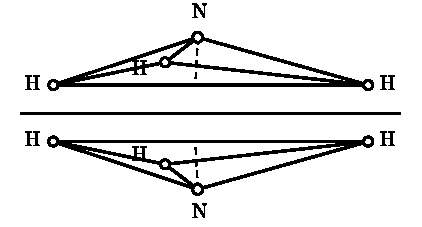
\includegraphics[width=6cm]{fig44.pdf}\\[0.3em]{\small 图 44}\end{minipage}\par\nopagebreak

球型陀螺式分子的例子，见本节题5.

\begin{xiti}
\setcounter{equation}{0}\renewcommand{\theequation}{\arabic{equation}}%

\noindent{\heiti 习题1}\quad 确立 $\mathrm{C_2^{12}H_4^1}$ 分子中态的对称性与该分子中氢核总自旋间的关系.

解：\footnote{应用置换群的方法求解类似的问题，可以考虑 I.~G.~Kaplan 的书（见§63），第6章，§2.}四个 $\mathrm{H}^1$ 核的总自旋可以具有 $I=2,1,0$ 三个值，它的投影 $M_I$ 可取2到 $-2$ 的各个值.我们从 $M_I$ 的最大值开始，逐个地考虑 $M_I$ 值相同的那些自旋因子所给出的表示.

$M_I=2$ 时只有一个自旋因子，其中所有原子核的自旋投影值都等于1/2.$M_I=1$ 时有四个不同的自旋因子，它们的区别在于四个原子核中一个核的自旋投影值等于 $-\dfrac{1}{2}$.最后，$M_I=0$ 时有六个不同的自旋因子，要看选取哪两个核的自旋投影值等于 $-\dfrac{1}{2}$.这三组自旋因子给出的三套群表示特征标如下表所示.
\begin{center}
\begin{tabular}{|c|c|c|c|c|c|c|c|c|}
\hline
  & $E$ & $\sigma(xy)$ & $\sigma(xz)$ & $\sigma(yz)$ & $I$ & $C_2(z)$ & $C_2(y)$ & $C_2(x)$\\ \hline
  $M_I=2$ & 1 & 1 & 1 & 1 & 1 & 1 & 1 & 1\\ \hline
  $M_I=1$ & 4 & 4 & 0 & 0 & 0 & 0 & 0 & 0\\ \hline
  $M_I=0$ & 6 & 6 & 2 & 2 & 2 & 2 & 2 & 2\\ \hline
\end{tabular}
\end{center}
第一个表示是单位表示 $A_g$；由于 $I=2$ 时才能有 $M_I=2$，因此 $A_g$ 型的态对应于自旋 $I=2$.

$M_I=1$ 时可以有 $I=1$ 和 $I=2$，第二个表示减去第一个表示后再把它分解成不可约表示，结果发现 $I=1$ 时有 $B_{1g},B_{2u},B_{3u}$ 三种态.

最后，$M_I=0$ 时可以具有 $M_I=1$ 的各个表示和 $I=0$ 的表示.第三个表示减去第二个表示后得到两个 $A_g$ 态，对应于自旋 $I=0$.

\noindent{\heiti 习题2}\quad 对 $\mathrm{C_2^{12}H_4^2},\mathrm{C_2^{13}H_4^1},\mathrm{N_2^{14}O_4^{16}}$ 分子，求总（坐标）波函数的对称类型及其相应能级的统计权重［所有这些分子具有同一形式，核自旋为 $i(\mathrm{H}^2)=1$，$i(\mathrm{C}^{13})=1/2$，$i(\mathrm{N}^{14})=1$］.

解：与本节所讲的 $\mathrm{C_2^{12}H_4^1}$ 分子的方法相同，求得下列各态（所选的坐标轴也和例中的一样）：
\begin{center}
\begin{tabular}{|c|c|c|}
\hline
  分\ 子 & $(+)$ & $(-)$\\ \hline
  $\mathrm{C_2^{12}H_4^2}$ & $27A_g,\ 18B_{1g}$ & $18B_{2u},\ 18B_{3u}$\\ \hline
  $\mathrm{C_2^{13}H_4^1}$ & $16A_g,\ 12B_{1g}$ & $12B_{2u},\ 24B_{3u}$\\ \hline
  $\mathrm{N_2^{14}O_4^{16}}$ & $6A_g$ & $3B_{3u}$\\ \hline
\end{tabular}
\end{center}

\noindent{\heiti 习题3}\quad 同上题，但分子为 $\mathrm{N^{14}H_3^2}$.

解：与本节中 $\mathrm{N^{14}H_3^1}$ 分子的做法一样，求得的态为 $30A_1,3A_2,24E$.对基态电子谱项最低振动能级讲来，不同的 $k$ 值具有下列各态：
\begin{center}
\begin{tabular}{|c|c|c|}
\hline
  & $(+)$ & $(-)$\\ \hline
  $|k|$不是3的倍数 & $24E$ & $24E$\\ \hline
  $|k|$是3的倍数 & $30A_1,3A_2$ & $30A_1,3A_2$\\ \hline
  $k=0\left\{\begin{array}{l}J\text{ 为偶数}\\ J\text{ 为奇数}\end{array}\right.$
  & $\begin{array}{c}30A_1\\ 3A_2\end{array}$
  & $\begin{array}{c}3A_2\\ 30A_1\end{array}$\\ \hline
\end{tabular}
\end{center}

\noindent{\heiti 习题4}\quad 与上题同，但分子为 $\mathrm{C_2^{12}H_6^1}$（见图43f；对称群为 $\boldsymbol{D}_{3d}$）.

解：可能态具有下列类型：$7A_{1g},1A_{1u},3A_{2g},13A_{2u},9E_g,11E_u$.

对基态电子谱项最低振动能级讲来，可得下列各态：
\begin{center}
\begin{tabular}{|c|c|c|}
\hline
  & $(+)$ & $(-)$\\ \hline
  $|k|$不是3的倍数 & $9E_g$ & $11E_u$\\ \hline
  $|k|$是3的倍数 & $7A_{1g},3A_{2g}$ & $1A_{1u},13A_{2u}$\\ \hline
  $k=0\left\{\begin{array}{l}J\text{ 为偶数}\\ J\text{ 为奇数}\end{array}\right.$
  & $\begin{array}{c}7A_{1g}\\ 3A_{2g}\end{array}$
  & $\begin{array}{c}1A_{1u}\\ 13A_{2u}\end{array}$\\ \hline
\end{tabular}
\end{center}

\noindent{\heiti 习题5}\quad 同上题，但为甲烷分子 $\mathrm{C^{12}H_4^1}$（C 原子在四面体中心，四个 H 原子在顶角）.

解：这个分子属于球型陀螺式，对称群为 $\boldsymbol{T}_d$.用同一方法可以求出可能态的类型为：$5A_2,1E,3F_1$（分子的总自旋相应地等于 $2,0,1$）.

球型陀螺的转动态是按总角动量 $J$ 值分类的.每个 $J$ 值有 $2J+1$ 个转动函数，给出了 $\boldsymbol{O}$ 群的一个 $2J+1$ 维表示，$\boldsymbol{O}$ 群与 $\boldsymbol{T}_d$ 群同构，它是把 $\boldsymbol{T}_d$ 群中的所有对称平面换成垂直于它的二阶轴后得到的.这个表示的特征标由(98.3)式所确定.例如 $J=3$ 时可得下列群表示特征标：
\begin{center}
\begin{tabular}{|c|c|c|c|c|}
\hline
  $E$ & $8C_3$ & $6C_2$ & $6C_4$ & $3C_4^2$\\ \hline
  $7$ & $1$ & $-1$ & $-1$ & $-1$\\ \hline
\end{tabular}
\end{center}
其中所含的 $\boldsymbol{O}$ 群不可约表示为 $A_2,F_1,F_2$.再来研究基态电子谱项最低振动能级的转动结构，所得的结论是，$J=3$ 时总波函数为 $A_2$ 型的能级只能是正的，$F_1$ 型态的能级则可正可负.对于前几个 $J$ 值，可得下列各态（它们的核统计权重也一起写出）：
\begin{center}
\begin{tabular}{|c|c|c|}
\hline
  & $(+)$ & $(-)$\\ \hline
  $J=0$ & —— & $5A_2$\\ \hline
  $J=1$ & $3F_1$ & ——\\ \hline
  $J=2$ & $1E$ & $1E,3F_1$\\ \hline
  $J=3$ & $5A_2,3F_1$ & $3F_1$\\ \hline
  $J=4$ & $1E,3F_1$ & $5A_2,1E,3F_1$\\ \hline
\end{tabular}
\end{center}

\end{xiti}
\renewcommand{\theequation}{\arabic{section}.\arabic{equation}}%
